%%
%% Copyright (c) 2018-2019 Weitian LI <liweitianux@sjtu.edu.cn>
%% Creative Commons BY 4.0
%%

\chapter{基于深度学习的再电离信号分离新算法}
\label{chap:cdae}

为了能够从强烈的前景干扰中分离出微弱的 EoR 信号,
传统的\ac{fg-rm}方法都依赖于一个关键的前提:
前景干扰具有非常光滑的频谱,而 EoR 信号沿频率维度发生剧烈变化,
两者具有显著不同的频谱结构,从而能够被有效地分离开 \cite{morales2010,chapman2016}.
然而,在实际情况中,未分辨的或者未完全扣除的干扰源在干涉阵列的波束效应的影响下,
会在频率维度产生震荡形式的辐射,破坏前景频谱的光滑性 \cite{liu2009ps}.
这会显著削弱前景干扰与 EoR 信号的可分性,
导致传统\ac{fg-rm}方法的效果大打折扣甚至失效,
因此需要研发能够克服波束效应的 EoR 信号分离新算法.


%=====================================================================
\section{波束的频率依赖效应}
\label{sec:beam-effect}

\begin{figure}[htp]
  \centering
  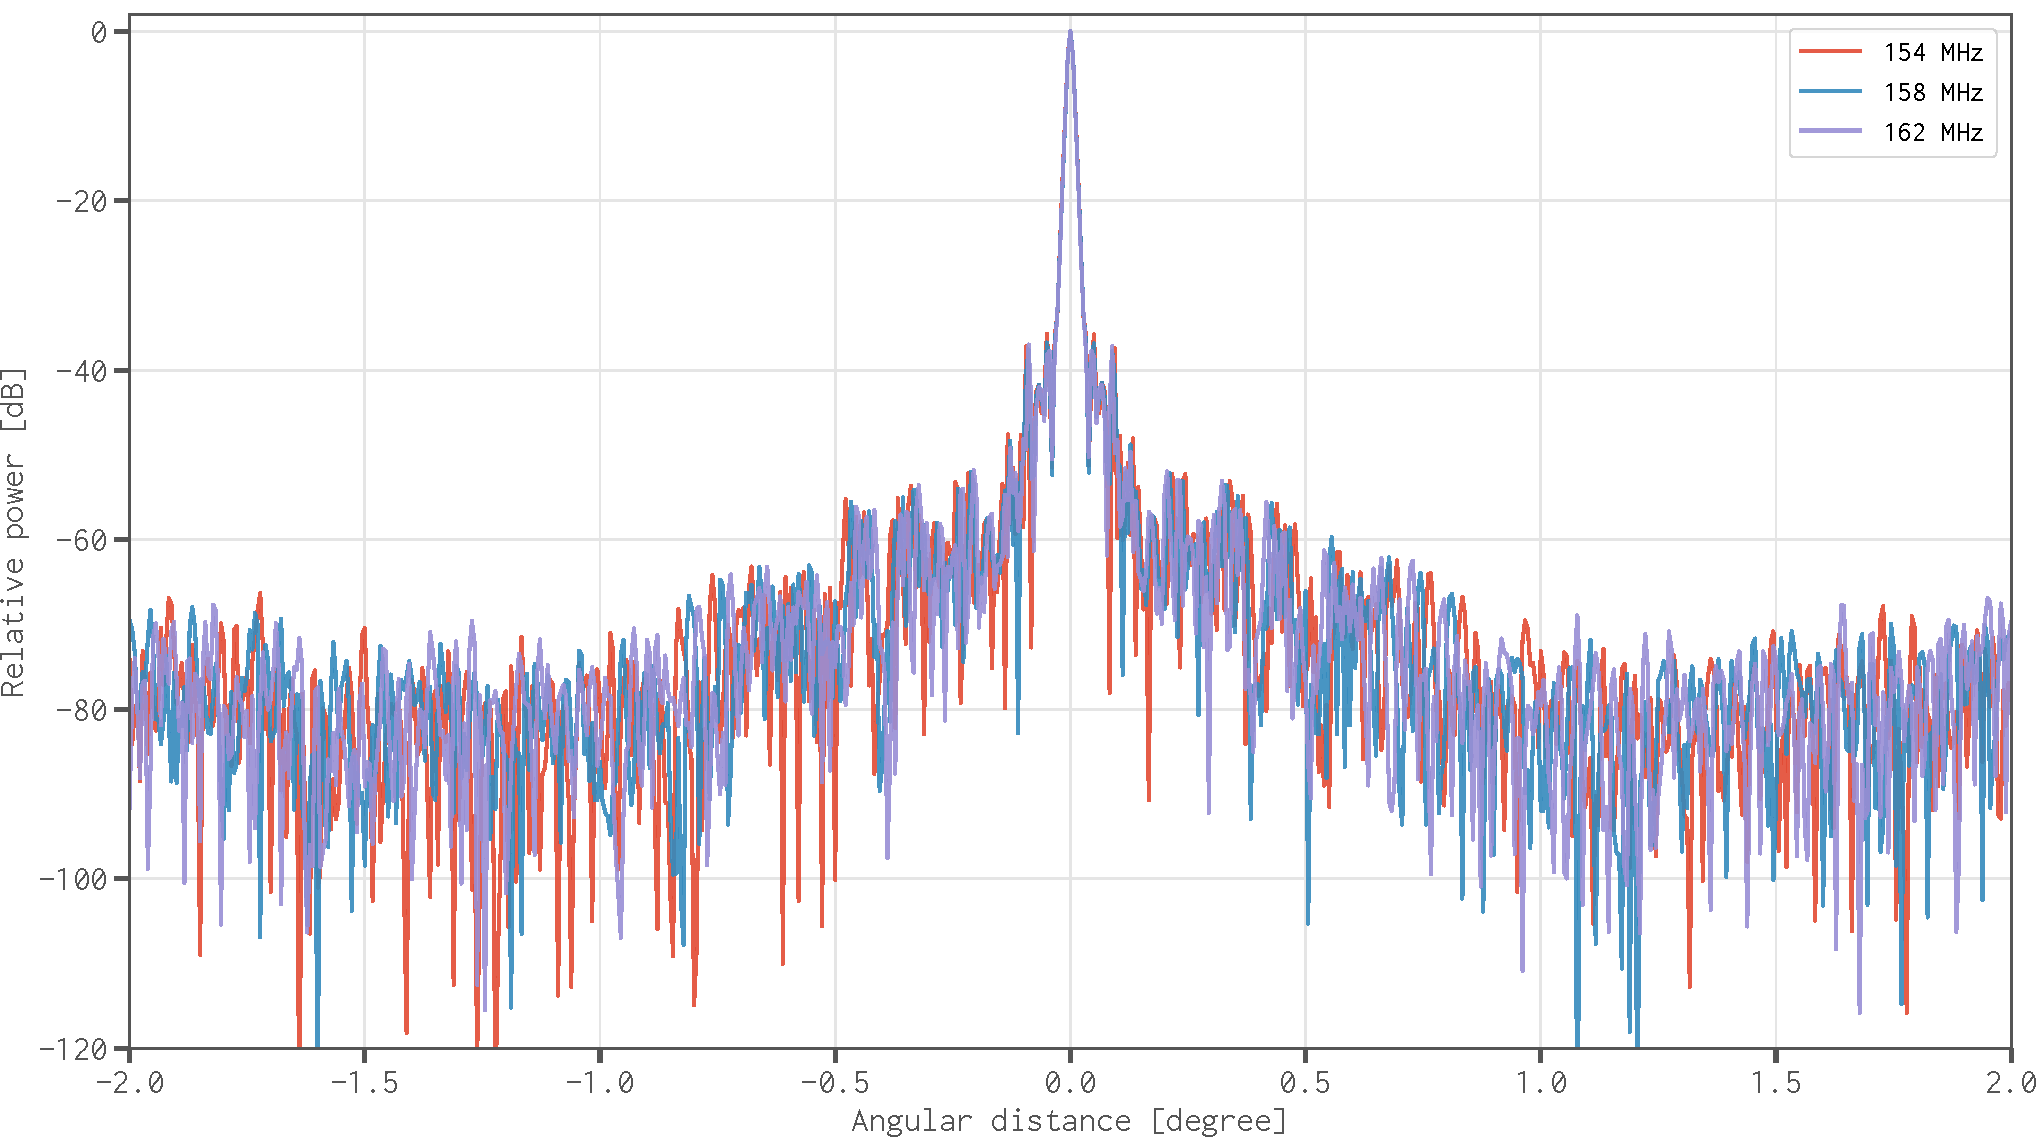
\includegraphics[width=\textwidth]{SKA1-low-psf}
  \bicaption[模拟的 SKA1-Low 综合波束]{%
    在 154、158 和 162 MHz 处模拟的 SKA1-Low \acs*{beam-synthesized}.
    积分时间为 \SI{6}{\hour}.
  }{%
    The simulated synthesized beams of SKA1-Low at 154, 158, and 162 MHz.
    The integration time is \SI{6}{\hour}.
  }
  \label{fig:ska-psf}
\end{figure}

一个干涉阵列拥有的\ac{baseline}的数目和长度均是有限的,
在观测中能实现的 $uv$ 覆盖也是有限而且不完备的 (\autoref{sec:uv-coverage}),
因此,干涉阵列的\ac{beam-synthesized}的形状非常复杂.
如\autoref{fig:ska-psf} 所示,
除了中间一个很窄的\ac{mainlobe},\ac{beam-synthesized}还包含一系列\ac{sidelobe}.
这些\ac{sidelobe}的数量非常多,相对幅度约为 \numrange{0.01}{0.1}\%,
一直延伸到远超出视场的位置.
另见 \citeay{liu2009ps} 的图 1 和图 3.

另一方面,\ac{beam-synthesized}的形状还依赖于观测频率.
\ac{sidelobe}的位置 $\theta$ 会随着频率 $\nu$ 的增大而向中间移动,
即 $\theta \propto \nu^{-1}$.
因此,一个干扰源在视场中所产生的辐射的位置也随频率而变化.
由于仪器的热噪声水平、成像的天区大小、CLEAN 的深度等因素的限制,
视场中总是存在一批未分辨的以及未完全扣除而残留的干扰源.
由这些干扰源的辐射综合而成的前景干扰,
在频率维度将出现类似\ac{beam-synthesized}的\ac{sidelobe}形状的起伏.
这将破坏前景辐射的频谱光滑性,使得前景干扰具有类似 EoR 信号的小尺度频谱结构,
导致传统\ac{fg-rm}方法无法有效地将两者区分开.
另见 \citeay{liu2009ps} \S\,1.


%=====================================================================
\section{基于深度学习的新算法}

鉴于\ac{beam-synthesized}的形状非常复杂,并且随频率和位置而变化,
即使付出昂贵的计算代价,
为传统\ac{fg-rm}方法手工打造一个用于克服上述波束效应的模型仍然非常困难
\cite{lochner2015}.
此外,SKA1-Low 等大型干涉阵列的海量数据的处理已经成为一个重要的瓶颈
\cite{norris2011,dolensky2016,chrysostomou2018},
所以采用传统\ac{fg-rm}方法并建模克服波束效应在实际应用中几乎不可行.
相比于传统方法,\ac{dl}方法能够自动地从数据中汲取信息用来优化模型;
一旦训练好模型,使用该模型则变得非常高效;
方法的灵活性高,只需要使用合适的数据重新训练,便可以将方法运用于其他望远镜.
因此,基于\ac{dl}研发能够克服波束效应的 EoR 信号分离算法更具有可行性和吸引力
\cite{herbel2018,vafaeiSadr2019}.

\begin{figure}[htp]
  \centering
  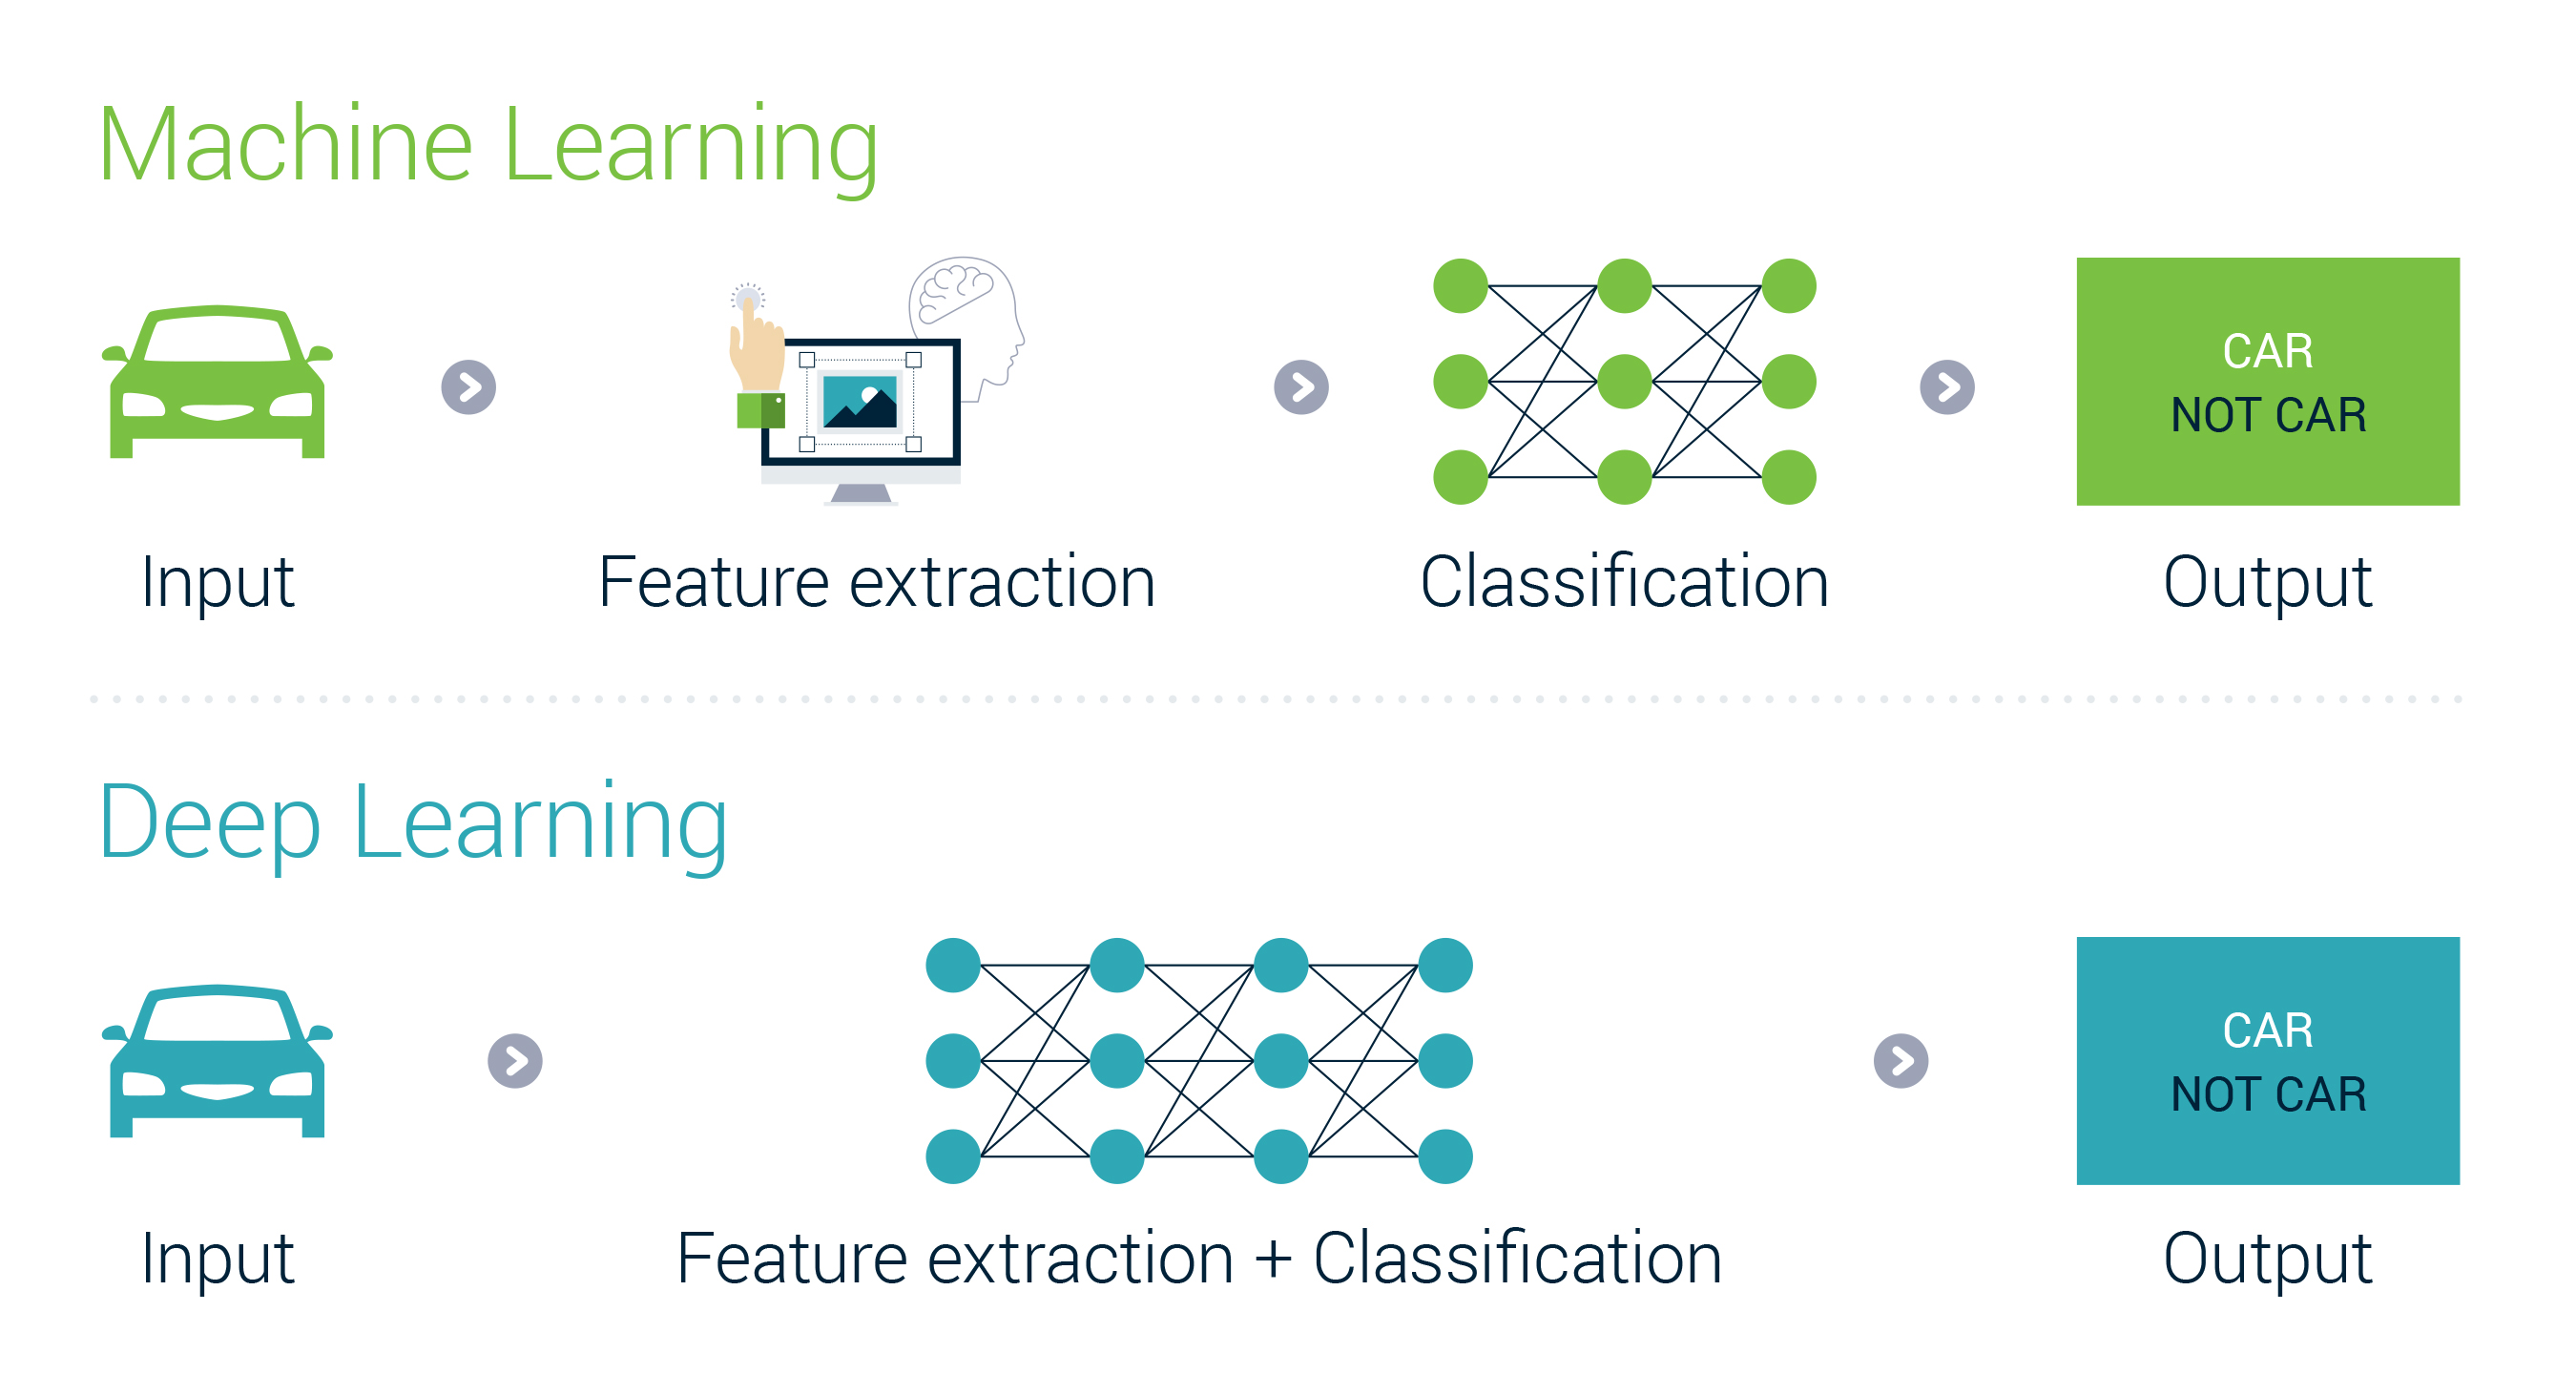
\includegraphics[width=\textwidth]{ml-vs-dl}
  \bicaption[机器学习和深度学习之间的主要区别]{%
    机器学习和深度学习之间的主要区别.
    深度学习拥有\acs*{fx}的能力,而不必手工设计需要从数据中提取的特征.
  }{%
    The main difference between machine learning and deep learning.
    The feature extraction is an integral part of the deep learning;
    therefore, there is no need to craft the features to be extracted
    from the data.
    \\来源/Credit:
    Jochem Grietens,
    \url{https://verhaert.com/difference-machine-learning-deep-learning/},
    (2019-04-25)
  }
  \label{fig:ml-dl}
\end{figure}

\ac{dl}是\ac{ml}的一个子集,同时后者又是\ac{ai}的一个子集.
\ac{ai}起始于上世纪 50 年代,该领域的开创人之一 John McCarthy 将\ac{ai}定义为
\enquote{制造智能机器的科学和工程} \cite{mcCarthy2007}.
早期的\ac{ai}系统完全基于一整套规则,而这些规则需要明确地由人来定义和实现
\cite{haugeland1985,jackson1998}.
\ac{ml}提供了另一条实现\ac{ai}的途径:
通过让机器从数据中学习并调整自身算法,达到解决\ac{ai}领域的问题的目标
\cite{samuel1959,mitchell1997}.
利用该方法,我们只需要设计机器需要从数据中提取的特征以及相应的学习策略,
而不需要编写每一条具体的规则,有效地减轻了开发\ac{ai}系统的负担.
\ac{dl}是\ac{ml}中的一个分支,
利用多层\ac{nn}架构让机器自己去发掘数据中的特征,
并从简单特征构建出复杂特征,学习得到数据的一个有效\ac{representation}
\cite{bengio2013rl,schmidhuber2015,goodfellow2016}.
换言之,\ac{dl}让机器自身拥有了\ac{fx}的能力,
从而进一步降低了开发先进的\ac{ai}系统的难度,
极大地拓展了\ac{ai}的应用范围.
\autoref{fig:ml-dl} 示意了\ac{ml}和\ac{dl}之间的主要区别.

近十多年以来,\ac{dl}发展迅猛,已经被应用到计算机视觉 (computer vision)、
语音识别 (speech recognition)、自然语言处理 (natural language processing)
等诸多领域,并取得了一系列突破性成果,
详见 \citeay{leCun2015} 综述文.
\ac{dl}算法包括多种\ac{nn} \cite{bengio2009,leCun2015,schmidhuber2015},
比如\ac{dnn}、\ac{cnn}、\ac{rnn}、\ac{ae}.
其中,\ac{ae}能够以\ac{unsupervised}的方式学习得到
输入数据的\ac{representation} \cite{bourlard1988},
因此经常被用于数据的\ac{dim-reduction}\cite{hinton2006,wang2014}
和\ac{denoising}\cite{xie2012,lu2013,bengio2013}.
在\ac{ae}的诸多变种中,\ac{cdae}尤其擅长于发掘数据中的抽象、细微的特征 \cite{du2017},
并且已经被成功地用于微弱\ac{gw}信号的\ac{denoising}\cite{shen2017}、
单声道音源的分离\cite{grais2017}、等等.

这些应用说明了 \ac{cdae} 具有从高度时变 (temporal-variable)
的数据中提取微弱信号的出色能力,
因此,值得尝试将 \ac{cdae} 应用于 EoR 信号的分离.
尽管待分离的 EoR 信号的\ac{snr}比上述应用中的情况更低,
但是 EoR 信号、前景辐射以及望远镜的波束效应都是稳定或近似稳定的.

%---------------------------------------------------------------------
\subsection{卷积去噪自编码器}
\label{sec:cdae}

\begin{figure}[htp]
  \centering
  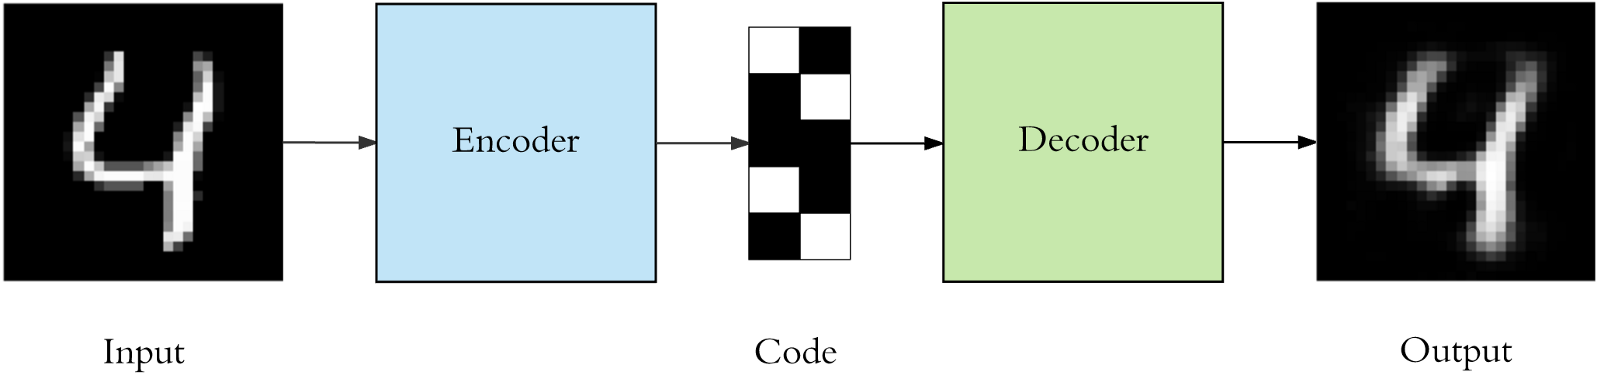
\includegraphics[width=0.8\textwidth]{autoencoder}
  \bicaption[自编码器的示意图]{%
    \acs*{ae}的示意图.
  }{%
    Diagram of an autoencoder.
    \\来源/Credit:
    Arden Dertat,
    \url{https://towardsdatascience.com/applied-deep-learning-part-3-autoencoders-1c083af4d798},
    (2019-04-25)
  }
  \label{fig:autoencoder}
\end{figure}

\emph{\ac{ae}}由\ac{encoder}和\ac{decoder}两部分组成,
其中\ac{encoder}将输入信号 $\B{x}$ 映射成一个内部\ac{code} $\B{h}$,
可表示为 $\B{h} = f(\B{x})$;
\ac{decoder}则尝试从\ac{code} $\B{h}$ 重建原输入信号,
可表示为 $\B{r} = g(\B{h})$;
如\autoref{fig:autoencoder} 所示.
因为我们将在频率维度对天空像素点逐个进行 EoR 信号的分离,
所以,输入信号 $\B{x}$ 表示一个天空像素点的频谱,
$\B{x}$、$\B{h}$ 和 $\B{r}$ 在本工作中均为一维矢量.
通过对\ac{code} $\B{h}$ 施加一定的约束(如限制其维度或稀疏性),
同时训练\ac{ae}使得重建信号 $\B{r}$ 与输入信号 $\B{x}$
之间的\ac{loss} $L(\B{r}, \,\B{x})$ 达到最小,
则\ac{ae}所学习到的\ac{code}将能有效地表示输入信号.
详见 \citeay{goodfellow2016}, 第 14 章.

\ac{ae}所学到的\ac{representation}的质量直接决定了\ac{ae}的性能.
为了促使\ac{ae}学习一个更好的\ac{representation},
\citeay{vincent2008} 和 \citeay{vincent2010}
基于\enquote{\ac{denoising}准则}提出了一种全新的训练策略:
首先人为地损坏(比如加入噪声)原始输入信号 $\B{x}$,
得到受损信号 $\B{x}'$ 并输入\ac{ae}进行训练,
使其重建信号 $\B{r}$ 尽可能地恢复原始输入信号 $\B{x}$,
即最小化\ac{loss} $L(\B{r}, \,\B{x})$.
这个\ac{denoising}过程迫使\ac{ae}发掘原始输入信号 $\B{x}$
中那些对准确重建起关键作用的稳健特征.
使用该\ac{denoising}准则训练的\ac{ae}也被称为\emph{\ac{dae}}.

\begin{figure}[htp]
  \centering
  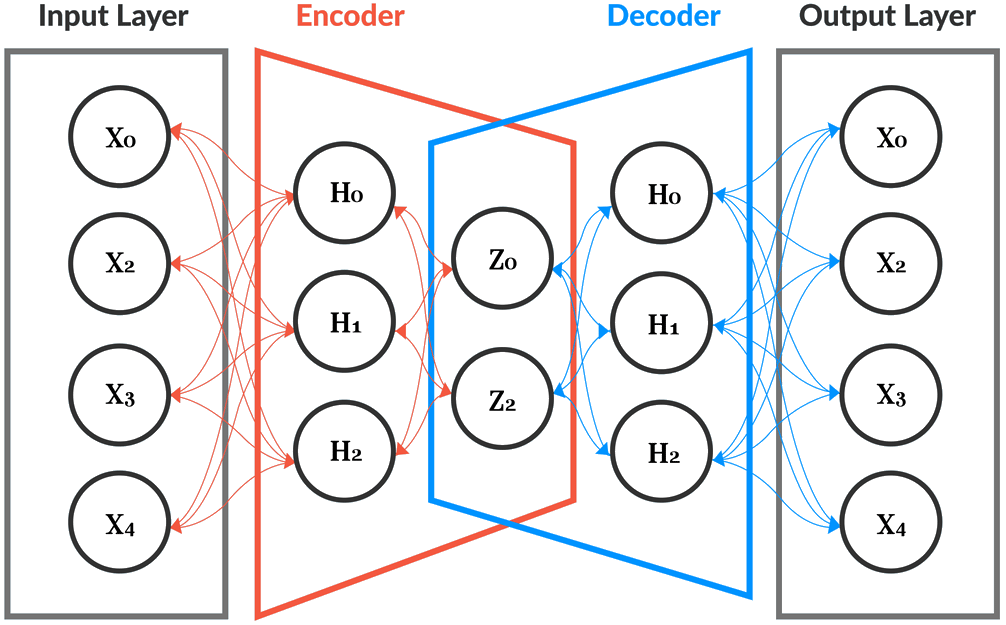
\includegraphics[width=0.6\textwidth]{autoencoder-fc}
  \bicaption[使用全连接层的经典自编码器的示意图]{%
    使用\acs*{fc}层的经典\acs*{ae}的示意图.
    \acs*{fc}层的每个\acs*{neuron}都与上一层的所有的\acs*{neuron}相连.
  }{%
    Diagram of a classic autoencoder that uses fully connected layers.
    Every neuron in a fully connected layer is connected to all neurons
    in the previous layer.
    \\来源/Credit:
    Trix Genota,
    \url{https://medium.com/@abien.agarap/implementing-an-autoencoder-in-tensorflow-2-0-5e86126e9f7},
    (2019-04-26)
  }
  \label{fig:autoencoder-fc}
\end{figure}

\begin{figure}[htp]
  \centering
  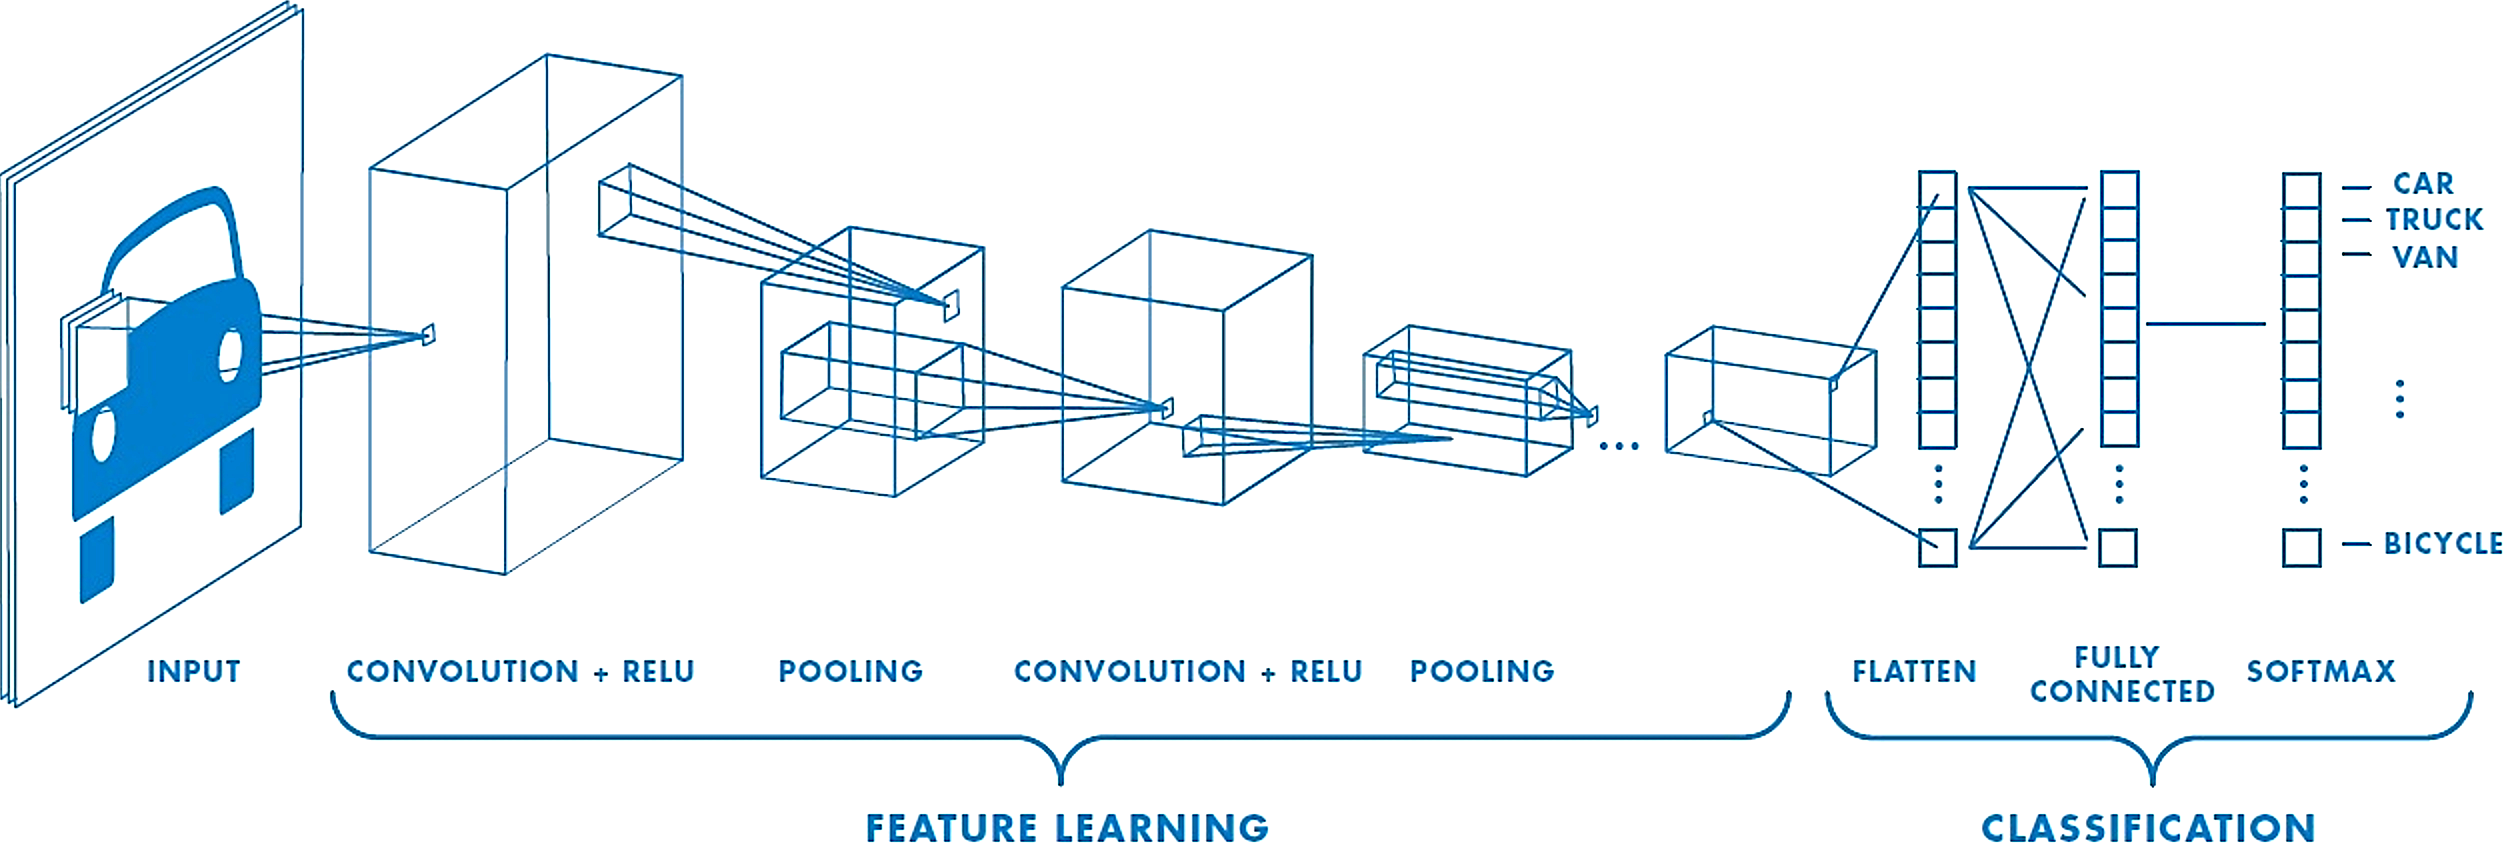
\includegraphics[width=\textwidth]{cnn}
  \bicaption[卷积神经网络的示意图]{%
    卷积神经网络的示意图,一般包括多个卷积层,
    每个卷积层由一组小尺寸\acs*{filter}构成,
    每个\acs*{filter}在数据的所有位置共享其参数.
  }{%
    Diagram of a convolutional neural network,
    which includes several convolutional layers.
    A convolutional layer consists of a set of small filters,
    each of which shares its weights among all locations in the data.
    \\来源/Credit:
    Sumit Saha,
    \url{https://towardsdatascience.com/a-comprehensive-guide-to-convolutional-neural-networks-the-eli5-way-3bd2b1164a53},
    (2019-04-26)
  }
  \label{fig:cnn}
\end{figure}

经典\ac{ae}由多个\ac{fc}层构成,其中每个\ac{neuron}都与上一层的所有\ac{neuron}相连,
如\autoref{fig:autoencoder-fc} 所示.
这种设计使\ac{ae}的参数数目随层数呈指数级增长,难以构建很深的网络.
此外,使用\ac{fc}层提取的特征是全局性的,
所以\ac{fc}层不适合用来学习输入数据中的局部特征(如图像中的文字、物体等),
而这些局部特征通常包含了数据的关键信息 \cite{masci2011}.
在另一方面,\ac{cnn}则使用多个卷积层来提取数据中的特征,如\autoref{fig:cnn} 所示.
每个卷积层由一组小尺寸(大小通常为 3、5、7)\ac{filter}构成,
每个\ac{filter}的权重参数不随数据的位置而变化.
这样,卷积层非常适合于提取数据中的局部特征 \cite{leCun1998},
同时有效地减少了参数数目.
\ac{cnn} 的参数数目通常约为类似的\ac{fc}\ac{nn}的 1\% 或更少 \cite{grais2017},
所以 \ac{cnn} 更容易训练,消耗的资源(如内存和时间)也更少.
另外,多个卷积层可以很容易地堆叠起来;
在前一层所提取的特征的基础上,更复杂、更抽象的特征能够从数据中提取出来.
这种技术推动我们设计出极深(几十层甚至上百层)、极富表达力的 \ac{cnn},
并且这些 \ac{cnn} 在图像分类及相关领域有着非凡的表现
\cite{krizhevsky2012,simonyan2014,szegedy2015,ma2019}.

\emph{\ac{cdae}} 是使用了多个卷积层而非\ac{fc}层的\ac{dae},
因此拥有和 \ac{cnn} 一样强大的\ac{fx}能力.
如此一来,\ac{cdae} 有能力从输入数据中学习一个更好的\ac{representation},
从而拥有更强的\ac{denoising}能力,能够重建即使严重受损的信号 \cite{du2017}.
所以,\ac{cdae} 非常适合用来发掘 EoR 信号和前景辐射之间的复杂区别,
进而实现两者的准确分离.

%---------------------------------------------------------------------
\subsection{网络架构}
\label{sec:architecture}

\begin{figure}[htp]
  \centering
  % Credit: https://tex.stackexchange.com/a/201120
  \rotatebox[origin=c]{90}{%
    \begin{minipage}{0.99\textheight}
      \centering
      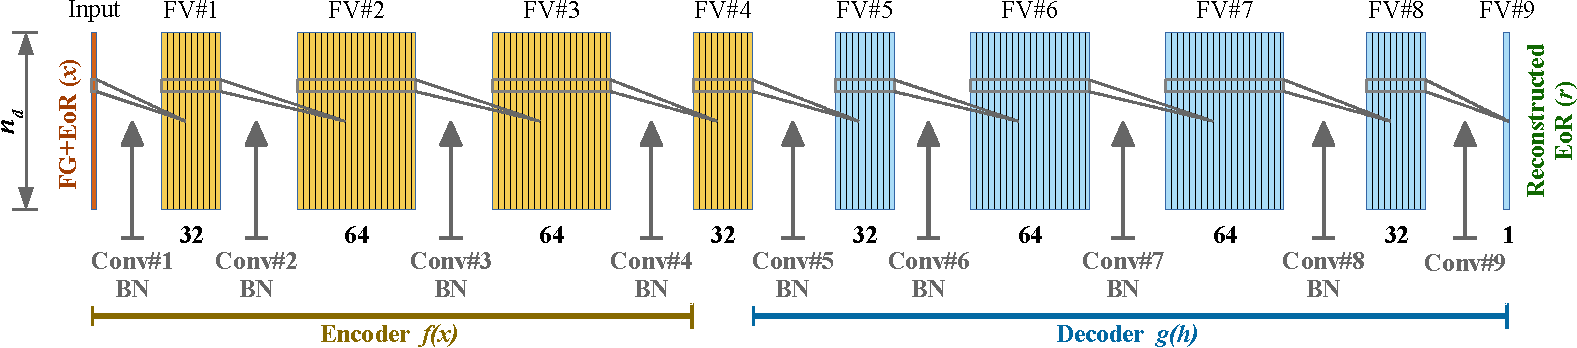
\includegraphics[width=\linewidth]{cdae-network-crop}
      \bicaption[CDAE 网络架构示意图]{%
        本文所提出的 CDAE 网络架构示意图,
        由一个四层的\acs*{encoder}和一个五层的\acs*{decoder}组成.
        黄色和蓝色方框分别表示\acs*{encoder}和\acs*{decoder}输出的\acs*{fv} (FV),
        方框下方的数字表示相应的卷积层所包含\acs*{filter}的数目.
        除了最后一层,其他层均使用了\acs*{batch-norm} (BN) 技术.
      }{%
        The architecture of the proposed CDAE that consists of a
        four-layer encoder and a five-layer decoder.
        The yellow and blue boxes represent the feature vectors (FV)
        generated by the encoder and decoder layers, respectively.
        The numbers marked below the boxes are the number of filters in
        the corresponding convolutional layers.
        The batch normalization (BN) technique is applied to all layers
        except for the last layer.
      }
      \label{fig:cdae-network}
    \end{minipage}
  }
\end{figure}

\ac{ae}的\ac{encoder}和\ac{decoder}部分均包含多个卷积层.
因为我们关注于\ac{ae}的\ac{fx}能力和\ac{denoising}能力,
而不关心所得\ac{code} $\B{h}$ 的具体形式,
所以\ac{encoder}和\ac{decoder}之间并没有明确的界线.
设第 $l$ 个卷积层包含 $m_l$ 个\ac{filter}
$\left(\left\{ k_{i}^{(l)} \right\};\, i = 1, 2, \cdots, m_l \right)$,
其中每个\ac{filter} $k_{i}^{(l)}$ 卷积前一层的输出,
得到一个\ac{fv} $\B{v}_{i}^{(l)}$:
\begin{equation}
  \label{eq:conv}
  \B{v}_{i}^{(l)} = \phi^{(l)} \left( \sum_{j=1}^{m_{l-1}}
    \B{v}_{j}^{(l-1)} * W_i^{(l)} + b_i^{(l)} \right) ,
    \quad i = 1, 2, \cdots, m_{l} ,
\end{equation}
其中
$W_i^{(l)}$ 和 $b_i^{(l)}$ 分别是\ac{filter} $k_{i}^{(l)}$
的权重和\ac{bias}参数,
$\phi^{(l)}(\cdot)$ 是当前第 $l$ 层的\ac{f-activation},
$\B{v}_{j}^{(l-1)}$ 为前一层的输出,
\enquote{$*$} 表示卷积运算.
于是,第 $l$ 层的输出为该层所有\ac{filter}的\ac{fv}所构成的集合
$\left(\left\{ \B{v}_{i}^{(l)} \right\};\, i = 1, 2, \cdots, m_l \right)$.

我们遵循\ac{dl}的推荐做法\cite{geron2017,suganuma2018} 来设计 \ac{cdae} 的架构.
具体而言,所有卷积层的\ac{filter}的尺寸为 3,
并且使用\ac{elu}作为\ac{f-activation} $\phi^{(l)}(\cdot)$ \cite{clevert2016},
除了最后一层(即\ac{ae}的输出层)的\ac{f-activation}为\ac{f-tanh} \enquote{tanh}
(参见 \autoref{sec:preprocessing}).
此外,除了最后的输出层,其他层均使用了\ac{batch-norm}技术 \cite{ioffe2015}.
该技术不仅可以加快训练速度,提高模型的准确率,
还能作为一个\ac{regularizer}预防\ac{overfitting} \cite{geron2017}.

为了确定 \ac{cdae} 的卷积层数目以及每个卷积层的\ac{filter}个数,
我们构建了许多个包含不同数量的卷积层和\ac{filter}的 \ac{cdae},
然后评估这些 \ac{cdae} 的性能(详见 \autoref{sec:cdae-results}),
最后,我们选取了一个性能足够好并且最简单的 \ac{cdae},
如\autoref{fig:cdae-network} 所示.
这个 \ac{cdae} 由一个四层的\ac{encoder}和一个五层的\ac{decoder}组成,
其中\ac{encoder}的四个卷积层分别包含 32、64、64 和 32 个\ac{filter},
\ac{decoder}的五个卷积层分别包含 32、64、64、32 和 1 个\ac{filter}.
我们也测试了在 \ac{cdae} 中包含\ac{pooling}层和\ac{upsampling}层,
但这些层对 \ac{cdae} 的性能影响可以忽略不计,
因此,我们最终设计的 \ac{cdae} (\autoref{fig:cdae-network}) 完全由卷积层构成,
也被称为\ac{fcn} \cite{long2015,springenberg2015}.

%---------------------------------------------------------------------
\subsection{训练和评估方法}
\label{sec:train-eval}

在一开始,\ac{cdae} 的全部参数(即所有层的\ac{filter}的权重和\ac{bias})
由 He 均匀初始器 (He uniform initializer)\cite{he2015} 初始化为随机值.
为了训练这些参数以获得一个有效的 \ac{cdae},需要以下三个\ac{ds} \cite{ripley1996}:
\begin{itemize}
  \item \ac{s-training}:
    用于拟合 \ac{cdae} 的待训练参数;
  \item \ac{s-validation}:
    一方面用于验证训练过程是否正常,比如没有出现\ac{overfitting};
    另一方面用来约束 \ac{cdae} 的\ac{hyperparam},
    比如层数和\ac{filter}的数目 (\autoref{sec:architecture});
  \item \ac{s-test}:
    仅仅在训练结束后用来评估 \ac{cdae} 的性能.
\end{itemize}
上述每一个\ac{ds}都包含许多的数据点
$\left( \B{x}^{(i)}, \,\B{x}^{(i)}_{\R{eor}} \right)$,
其中 $\B{x}^{(i)}_{\R{eor}}$ 是一个天空像素点 $i$ 的 EoR 信号的频谱,
$\B{x}^{(i)} = \B{x}^{(i)}_{\R{eor}} + \B{x}^{(i)}_{\R{fg}}$
是该像素点的总辐射(前景辐射与 EoR 信号之和)的频谱.

在每一个训练\ac{epoch},将总辐射 $\B{x}^{(i)}$ 输入 \ac{cdae},
经过一系列卷积层 [\autoref{eq:conv}]
后得到重建的 EoR 信号 $\B{r}^{(i)}_{\R{eor}}$.
该重建信号 $\B{r}^{(i)}_{\R{eor}}$ 与输入的 EoR 信号 $\B{x}^{(i)}_{\R{eor}}$
之间的差异就是 \ac{cdae} 的\acl{loss} \ac{loss},
可利用\ac{mse}将其量化为:
\begin{equation}
  \label{eq:loss}
  \ac{loss} = \frac{1}{N_{\R{tr}}} \sum_{i=1}^{N_{\R{tr}}}
    \left[ \B{r}_{\R{eor}}^{(i)} - \B{x}_{\R{eor}}^{(i)} \right]^T
    \left[ \B{r}_{\R{eor}}^{(i)} - \B{x}_{\R{eor}}^{(i)} \right] ,
\end{equation}
其中 $N_{\R{tr}}$ 是\acl{s-training} \ac{s-training} 所包含数据点的数目,
\enquote{$T$} 表示\ac{transpose}算符.
运用\ac{backprop}方法\cite{rumelhart1986,leCun1998bp},
可以计算\acl{loss} \ac{loss} 对任意一个参数 $p_i$ 的梯度
$\partial \ac{loss} / \partial p_i$,
然后据此更新这些参数,使得\acl{loss} \ac{loss} 逐渐减小,
从而提高重建的 EoR 信号 $\B{r}^{(i)}_{\R{eor}}$ 的质量.
随着训练\ac{epoch}的增长,原来一个随机的 \ac{cdae} 被逐渐塑造成一个专用网络,
能够发掘输入数据中的有用特征并用来重建 EoR 信号.

为了定量评估已训练好的 \ac{cdae} 的性能,
我们采用 Pearson \acl{coef-correlation} (correlation coefficient)
\cite{harker2009,chapman2013}
来计算由 \ac{cdae} 重建的 EoR 信号 $\B{r}_{\R{eor}}$ 与输入 EoR 信号
$\B{x}_{\R{eor}}$ 之间的相似程度:
\begin{equation}
  \label{eq:corrcoef}
  \ac{coef-correlation}(\B{r}_{\R{eor}}, \B{x}_{\R{eor}})
      = \frac{\sum_{j=1}^{n}(r_{\R{eor},j} - \bar{r}_{\R{eor}})
            (x_{\R{eor},j} - \bar{x}_{\R{eor}})}{
          \sqrt{\sum_{j=1}^{n}(r_{\R{eor},j} - \bar{r}_{\R{eor}})^2
            \sum_{j=1}^{n}(x_{\R{eor},j} - \bar{x}_{\R{eor}})^2}
        } ,
\end{equation}
其中
$\bar{r}_{\R{eor}}$ 和 $\bar{x}_{\R{eor}}$ 分别表示
$\B{r}_{\R{eor}}$ 和 $\B{x}_{\R{eor}}$ 的平均值,
$n$ 是信号的长度.
\acl{coef-correlation}
$\ac{coef-correlation}(\B{r}_{\R{eor}}, \B{x}_{\R{eor}})$ 越接近于 1,
则表示重建的 EoR 信号越准确,\ac{cdae} 的性能也就越好.


%=====================================================================
\section{新算法的演示}
\label{sec:cdae-demo}

为了演示和评估基于\ac{dl}的新算法
(即我们在 \autoref{sec:architecture} 设计的 \ac{cdae})的性能,
我们首先针对 SKA1-Low 模拟得到\enquote{观测}图像 (\autoref{sec:cdae-images}),
然后对模拟图像进行预处理,生成 \ac{cdae} 所需的\ac{ds} (\autoref{sec:preprocessing}),
接着训练 \ac{cdae} 并评估其性能 (\autoref{sec:cdae-results}),
最后进一步验证 \ac{cdae} 的学习能力和效果 (\autoref{sec:cdae-validation}).

%---------------------------------------------------------------------
\subsection{观测图像模拟}
\label{sec:cdae-images}

取 \SIrange{154}{162}{\MHz} 这一典型频带为例 \cite{datta2010},
将其分成 $n_f = 101$ 个宽度为 \SI{80}{\kHz} 的频率\ac{channel}.
相比 \autoref{sec:obs-simu},
我们将频率分辨率从 \SI{160}{\MHz} 提高到了 \SI{80}{\MHz},
这样能够保留更多的频谱信息,有助于 EoR 信号的分离.

利用已在\autoref{chap:simulation}中详细描述的方法,
我们模拟了 EoR 信号 (\autoref{sec:simu-eor})
和前景辐射在每一个频率\ac{channel}里的\ac{skymap}.
其中前景辐射包括了银河系的\ac{rad-syn}和\ac{rad-ff} (\autoref{sec:simu-galactic})、
河外点源 (\autoref{sec:simu-eg-point})
以及星系团射电晕 (\autoref{sec:simu-halos}).
所有\ac{skymap}覆盖的天区大小为 \SI{10 x 10}{\degree},
图像尺寸为 \num{1800 x 1800},对应于 \SI{20}{\arcsecond} 的像素大小.

\begin{figure}[htp]
  \centering
  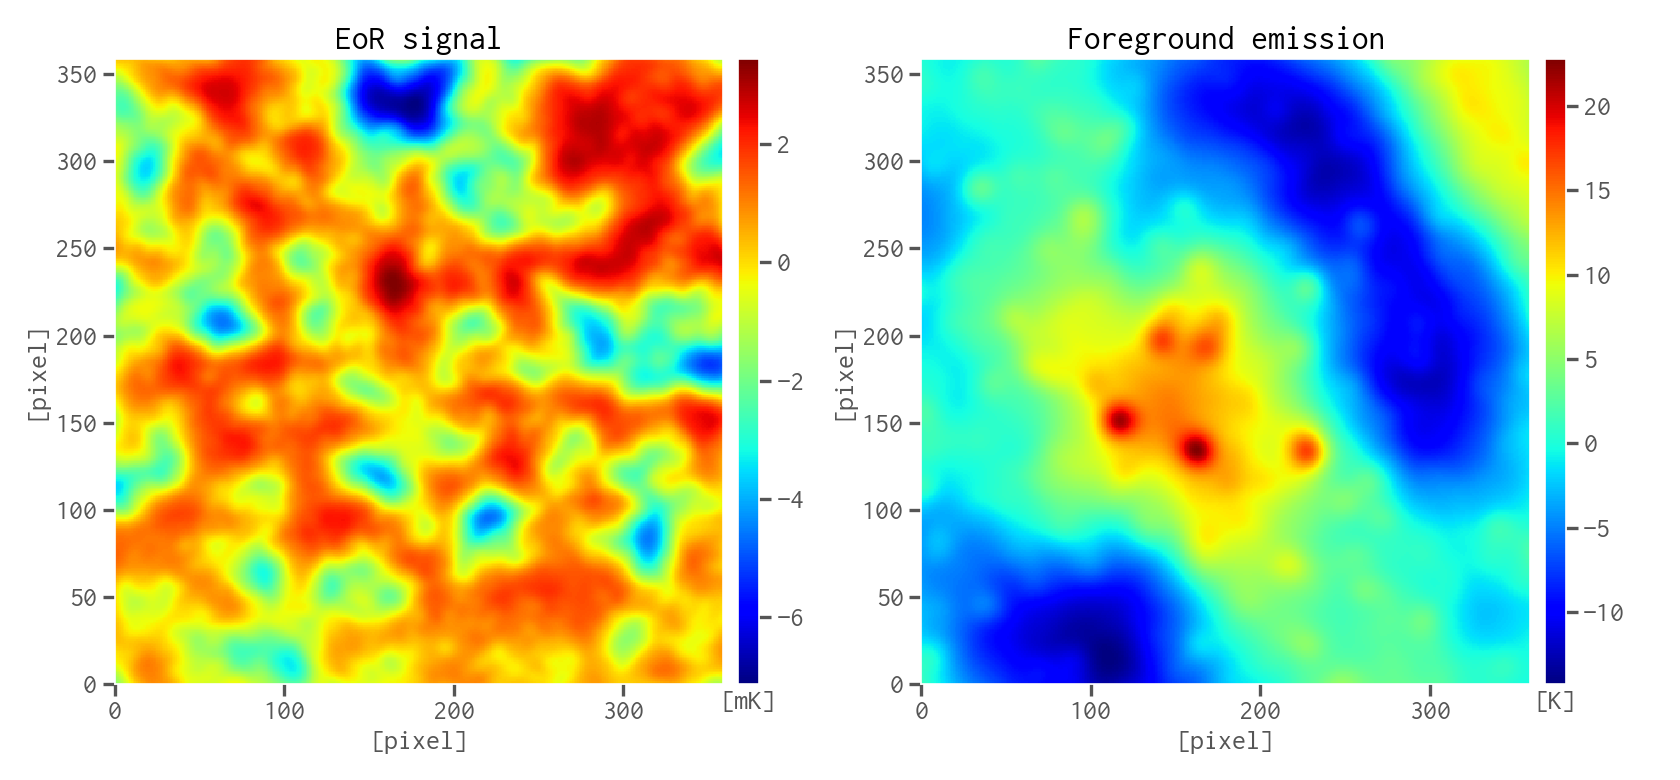
\includegraphics[width=\textwidth]{eor-fg-obsimg-158}
  \bicaption[EoR 信号和前景辐射在 \SI{158}{\MHz} 的模拟图像]{%
    EoR 信号(左栏)和前景辐射(右栏)在 \SI{158}{\MHz} 的模拟图像.
    两张图像的尺寸均为 \num{360 x 360} 并且覆盖天区的大小均为  \SI{2 x 2}{\degree}.
    右栏前景辐射图像中的斑点为明亮的点源和射电晕.
  }{%
    Simulated images of the EoR signal (left panel) and the foreground
    emission (right panel) at \SI{158}{\MHz}.
    Both images have sizes of \num{360 x 360} and cover sky areas of
    \SI{2 x 2}{\degree}.
    The blobs in the right panel show the bright point sources and radio
    halos.
  }
  \label{fig:eor-fg-obsimg}
\end{figure}

为了在模拟的\ac{skymap}中整合实际的波束效应,
我们按照 \autoref{sec:obs-simu} 所述方法对\ac{skymap}开展模拟观测,
获得了 SKA1-Low 的\enquote{观测}图像.
不过,我们根据这里的具体需求对 \autoref{sec:obs-simu} 的模拟方法进行了若干微调,
具体如下:
\begin{itemize}
  \item 因为我们只区分 EoR 信号和前景辐射,
    所以将所有前景成分的\ac{skymap}叠加起来再输入 \texttt{OSKAR} 模拟;
  \item 假定 \SI{158}{\MHz} 流量密度 $S_{158} > \SI{10}{\mJy}$
    的河外点源已被全部去除 \cite{liu2009ps};
  \item 为了强调暗弱而且比较弥散的 EoR 信号,
    我们在使用 \texttt{WSClean} 成像时选择了自然权重 (natural weighting),
    同时将基线范围限制在 \numrange{30}{1000} 个波长;
  \item 为了得到最佳的图像质量,我们只切取中央 \SI{2 x 2}{\degree}
    的区域,对应的图像尺寸为 \num{360 x 360}.
\end{itemize}
这样,我们得到了一对尺寸为 \num{360 x 360 x 101} 的\ac{imgcube}:
EoR 信号 $C_{\R{eor}}^{(1)}$ 和前景辐射 $C_{\R{fg}}^{(1)}$.
\autoref{fig:eor-fg-obsimg} 展示了两者在中心频率 \SI{158}{\MHz} 的模拟图像.

为了突出显示波束效应对前景辐射的频谱的影响,我们随机地选取一个天空像素点为例,
然后对比有无波束效应的情况下前景辐射的频谱变化,如\autoref{fig:cdae-simdata} 所示,
其中还显示了相应的差分频谱(即相邻两个频谱\ac{channel}的差值)以及 EoR 信号的频谱.
可以看出,前景辐射的本征频谱是非常光滑的(上栏),
但是在复杂的波束效应的影响下出现了许多小幅度、小尺度 ($<$\,\SI{1}{\MHz}) 的涨落(中栏),
因此,频谱的光滑性受到了严重损坏.
尽管这些小尺度的涨落与 EoR 信号(下栏)具有一些相似的频谱特征,
但两者之间仍然具有足够的可区分度,可以被 \ac{cdae} 发掘出来并用于 EoR 信号的分离.
此外,\autoref{fig:cdae-simdata} 还显示出\enquote{观测}的前景辐射(中栏)
的强度相比原来的理想情况(上栏)约小 2 个数量级,
导致这个差异的主要原因是因为干涉阵列无法测量天空辐射的绝对强度,
只能响应辐射的空间涨落 \cite{braun1985}.

\begin{figure}[htp]
  \centering
  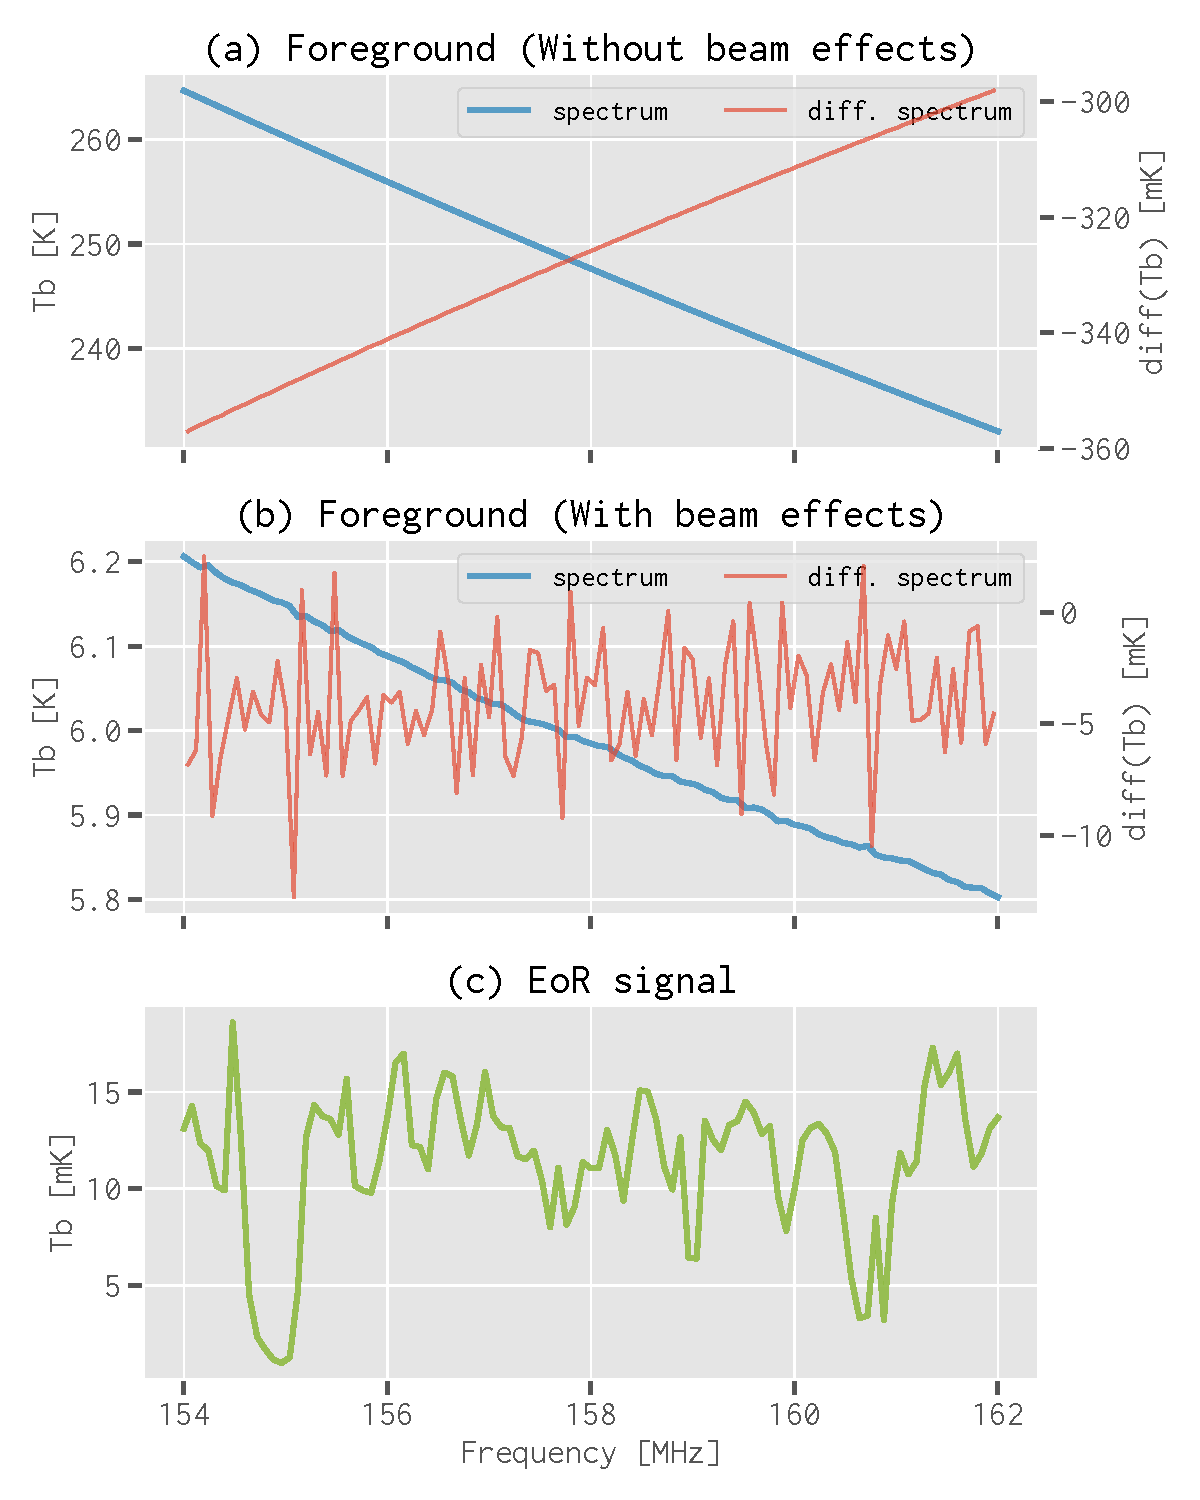
\includegraphics[width=0.84\textwidth]{cdae-simdata-example}
  \bicaption[前景辐射和 EoR 信号的频谱示例]{%
    随机取一个天空像素点为例,得到的前景辐射和 EoR 信号的频谱.
    \uline{(上栏)}
    理想的(即没有波束效应)前景辐射频谱(蓝线)以及相应的差分频谱(红线).
    \uline{(中栏)}
    仪器\enquote{观测}的(即包含波束效应)前景辐射频谱(蓝线)以及相应的差分频谱(红线).
    \uline{(下栏)}
    EoR 信号的频谱(绿线).
  }{%
    Example spectra of the foreground emission and the EoR signal for one
    random sky pixel.
    \emph{(Upper)} The ideal (i.e., without beam effects) foreground
    spectrum (blue line) and the corresponding differential spectrum
    (red line).
    \emph{(Middle)} The \enquote{observed} (i.e., with beam effects)
    foreground spectrum (blue line) and the corresponding
    differential spectrum (red line).
    \emph{(Lower)} The EoR signal spectrum (green line).
  }
  \label{fig:cdae-simdata}
\end{figure}

训练和评估 \ac{cdae} 需要三个\ac{ds},
分别为\acl{s-training}、\acl{s-validation} 和\acl{s-test}
(\autoref{sec:train-eval}),
如果只有一对\ac{imgcube},那么\acl{s-test} \ac{s-test} 只能包含一小部分的像素点的数据,
而且这些像素点随机地分布在天空平面里.
在 \ac{cdae} 的测试阶段 (\autoref{sec:cdae-results}),
利用这样一个\acl{s-test} \ac{s-test} 重建得到的 EoR 信号无法构成完整的
(甚至局部完整的)\ac{imgcube},
从而无法通过图像和\ac{ps}直观地展示 \ac{cdae} 分离 EoR 信号的效果.
因此,为\acl{s-test} \ac{s-test} 再额外模拟一对\ac{imgcube}能够解决上述问题.
由于最终经过切取的\ac{imgcube}所覆盖的天区大小仅有 \SI{2 x 2}{\degree},
我们设第二对\ac{imgcube}的中心坐标为
(R.A., Dec.\@) = (\SI{3}{\degree}, \SI{-27}{\degree}),
即与第一对\ac{imgcube}
$\left( C_{\R{eor}}^{(1)}, C_{\R{fg}}^{(1)} \right)$
的中心相距 \SI{3}{\degree}.
具体而言,我们以 (R.A., Dec.\@) = (\SI{3}{\degree}, \SI{-27}{\degree})
为中心模拟了银河系弥散辐射(\ac{rad-syn}和\ac{rad-ff})的\ac{skymap};
因为河外点源、射电晕以及 EoR 信号的空间分布几乎是各向同性的,
所以我们将它们原来的\ac{skymap}平移 \SI{3}{\degree} 得到所需的新\ac{skymap}.
然后,遵循相同的模拟观测方法,我们得到了第二对\ac{imgcube}
$\left( C_{\R{eor}}^{(2)}, C_{\R{fg}}^{(2)} \right)$.

鉴于我们的新算法是针对 EoR \ac{tomography}而设计的,
要求极深度的观测以达到足够低的噪声水平.
比如,SKA1-Low 计划筛选 5 个 EoR 天区,然后对每个天区观测约 \SI{1000}{\hour},
达到空前的约小于 \SI{1}{\mK} 的亮度灵敏度 [\autoref{eq:sigma-tb}],
从而实现 EoR 区域的直接成像观测 \cite{mellema2013,mellema2015,koopmans2015}.
因此,我们没有在上述模拟中包含仪器的热噪声.

%---------------------------------------------------------------------
\subsection{数据预处理}
\label{sec:preprocessing}

按照天空像素点将 \autoref{sec:cdae-images} 模拟得到的\ac{imgcube}重新组织,
形成一系列数据点 $\left( \B{x}^{(i)}, \,\B{x}^{(i)}_{\R{eor}} \right)$,
其中 $\B{x}^{(i)}_{\R{eor}}$ 和
$\B{x}^{(i)} = \B{x}^{(i)}_{\R{eor}} + \B{x}^{(i)}_{\R{fg}}$
分别表示像素点 $i$ 的 EoR 信号和总辐射的频谱.
数据点的总数为 $N_S = \num{360x360 x 2} = \num{259200}$,
这些数据点组成了训练和评估 \ac{cdae} 所需的\ac{ds}
$S = \left\{ \left(\B{x}^{(i)}, \,\B{x}^{(i)}_{\R{eor}} \right) \right\}$.
但是,\ac{cdae} 在使用该数据集 $S$ 时,
需要分别对输入的总辐射 $X = \big\{ \B{x}^{(i)} \big\}$
以及 EoR 信号 $X_{\R{eor}} = \big\{ \B{x}^{(i)}_{\R{eor}} \big\}$
进行合适的预处理.

对于输入数据 $X = \big\{ \B{x}^{(i)} \big\}$,
我们提出首先对信号 $\B{x}^{(i)}$ 进行 Fourier 变换.
这样可以提高 EoR 信号与前景辐射之间的可分度,
于是 \ac{cdae} 能够更容易、更好地学习两者之间的差异.
(我们将在 \autoref{sec:why-ft} 讨论不使用 Fourier 变换预处理数据时所得到的结果.)
由于信号 $\B{x}^{(i)}$ 的长度为 $n_f = 101$ 是有限的,
为了抑制信号的边界效应使 Fourier 变换产生显著的\ac{sidelobe}
(\autoref{sec:eval-method}),
我们在 Fourier 变换前对信号 $\B{x}^{(i)}$ 施加 Blackman--Nuttall \ac{f-window}
\cite{chapman2016} [\autoref{eq:bn-window}].
因为信号 $\B{x}^{(i)}$ 全部由实数组成,
所以变换后的 Fourier 系数 $\hat{x}^{(i)}_{f}$ 具有以下对称关系:
\begin{equation}
  \hat{x}^{(i)}_{f} \equiv \hat{x}^{*(i)}_{-f} ,
\end{equation}
其中 $f$ 表示 Fourier 频率,\enquote{$*$} 为\ac{conjugate}算符.
因此,只需要保留一半的 Fourier 系数即可.
于是,长度为 $n_f = 101$ 的信号 $\B{x}^{(i)}$ 变换为
$n_c = 51$ 个复 Fourier 系数:
\begin{equation}
  \left( \hat{x}^{(i)}_f; \; f = 0, 1, \cdots, 50 \right) ,
\end{equation}
其中,Fourier 频率 $f$ 最小的几个系数主要由频谱光滑的前景辐射贡献,
因此可以通过排除这几个 Fourier 系数来抑制前景干扰.
为了平衡前景辐射的抑制效果和 EoR 信号的损失程度,
经过测试,我们选择排除 $n_{\R{ex}} = 6$ 个 Fourier 频率最小的系数,
于是剩下的 45 个 Fourier 系数为:
\begin{equation}
  \left( \hat{x}^{(i)}_f; \; f = 6, 7, \cdots, 50 \right) .
\end{equation}
因为 \ac{cdae} 只能处理实数,
所以我们将这些复 Fourier 系数的实部和虚部分开,
设 $\hat{x}^{(i)}_f = a_f + \Ci\,b_f$,
然后重新拼接成一个长度为 $n_d = 90$ 的实矢量:
\begin{equation}
  (a_6, a_7, \cdots, a_{49}, a_{50},
   b_{50}, b_{49}, \cdots, b_7, b_6) .
\end{equation}
最后,将数据标准化,使其平均值为 0、标准差为 1.

对于输入的 EoR 信号 $X_{\R{eor}} = \big\{ \B{x}^{(i)}_{\R{eor}} \big\}$,
我们首先使用与上述 $X$ 相同的预处理方法:
进行 Fourier 变换,接着去除 $n_{\R{ex}}$ 个 Fourier 频率最小的系数,
再将复 Fourier 系数的实部和虚部拼接成实矢量.
后续的预处理步骤则与 $X$ 的预处理方法有所不同.
计算数据的第 1 和第 99 \ac{percentile},
然后将小于第 1 \ac{percentile}以及大于第 99 \ac{percentile}的元素截断,
用来防止数据中可能存在的\ac{outlier}阻碍 \ac{cdae} 的训练.
最后,将数据除以其最大绝对值,使其数值范围为 $[-1, 1]$.
这种处理方法允许我们在 \ac{cdae} 的输出层使用值域同样为 $[-1, 1]$
的 \enquote{tanh} 函数作为\ac{f-activation} (\autoref{sec:architecture}).

%---------------------------------------------------------------------
\subsection{训练和结果}
\label{sec:cdae-results}

从第一对\ac{imgcube}
$\left( C_{\R{eor}}^{(1)}, C_{\R{fg}}^{(1)} \right)$
预处理得到的数据被随机地划分为:
\begin{itemize}
  \item \acl{s-training} \ac{s-training}:
    包含 \num{103680} 个数据点,对应于一个\ac{imgcube}中 80\% 的像素点;
  \item \acl{s-validation} \ac{s-validation}:
    包含余下的 \num{25920} 个数据点,对应于 20\% 的像素点.
\end{itemize}
从第二对\ac{imgcube}
$\left( C_{\R{eor}}^{(2)}, C_{\R{fg}}^{(2)} \right)$
预处理得到的数据全部作为\acl{s-test} \ac{s-test},
即包含 \num{129600} 个数据点.
使用完整的\ac{imgcube}作为\acl{s-test}允许我们在测试 \ac{cdae}
的性能时能够获得重建 EoR 信号的完整图像.

我们使用了 \href{https://keras.io}{\texttt{Keras}}\footnote{%
  Keras: \url{https://keras.io} (v2.2.4)}
框架\cite{keras}来实现 \ac{cdae};
\texttt{Keras} 的后端支持为 Google
\href{https://www.tensorflow.org}{\texttt{TensorFlow}}\footnote{%
  TensorFlow: \url{https://www.tensorflow.org} (v1.12.0)}
\cite{tensorflow},
并且通过 NVIDIA
\href{https://developer.nvidia.com/cuda-zone}{\texttt{CUDA}}\footnote{%
  CUDA: \url{https://developer.nvidia.com/cuda-zone} (v9.1.85)}
来利用 \ac{gpu} 加速 \ac{cdae} 的训练.
我们采用了 Adam 优化方法\cite{kingma2015} 来训练 \ac{cdae},
初始\ac{learning-rate} 设为 $\alpha = \num{e-5}$,
\ac{batch-size} 取为 100.
然后在\acl{s-training} \ac{s-training} 上训练 \ac{cdae},
直到\acl{loss-training} \ac{loss-training} 收敛为止.
如\autoref{fig:cdae-train} 所示,训练过程持续了约 50 个\ac{epoch}.

\begin{figure}[htp]
  \centering
  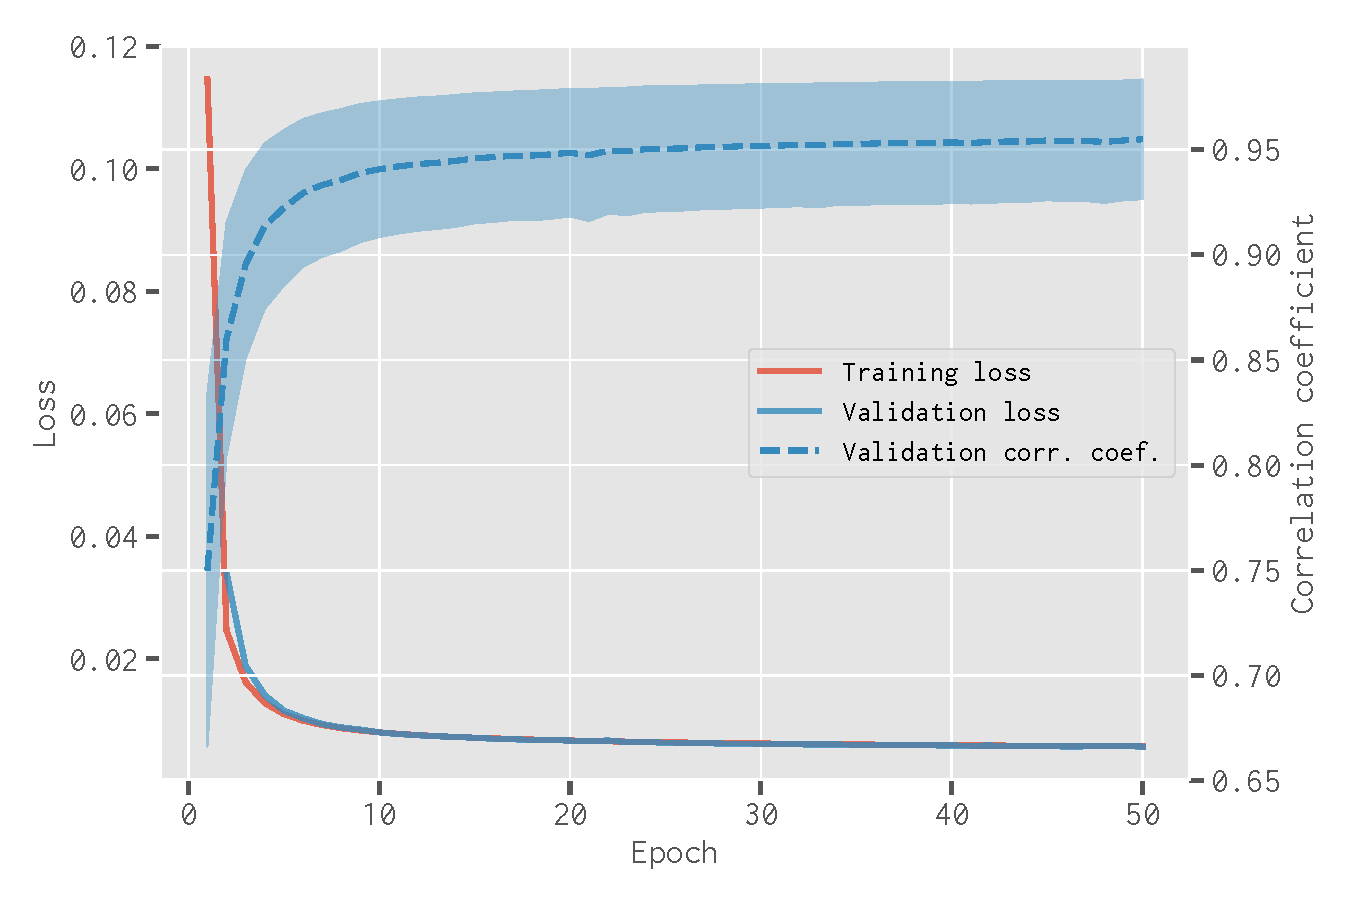
\includegraphics[width=\textwidth]{cdae-train}
  \bicaption[CDAE 的训练过程和结果]{%
    CDAE 的训练过程和结果.
    红色和蓝色实线分别显示了\acl*{loss-training} \ac*{loss-training}
    和\acl*{loss-validation} \ac*{loss-validation} 随训练过程的变化情况.
    蓝色虚线及其阴影区域分别表示从\acl*{s-validation} \ac*{s-validation}
    计算得到的\acl*{coef-correlation} \ac*{coef-correlation} 及其标准差.
  }{%
    The training loss \ac*{loss-training} (solid red line),
    validation loss \ac*{loss-validation} (solid blue line),
    and correlation coefficient \ac*{coef-correlation} (dashed blue line
    with shaded region representing its standard deviation) calculated on
    the validation set \ac*{s-validation} along the training of the CDAE.
  }
  \label{fig:cdae-train}
\end{figure}

\begin{figure}[htp]
  \centering
  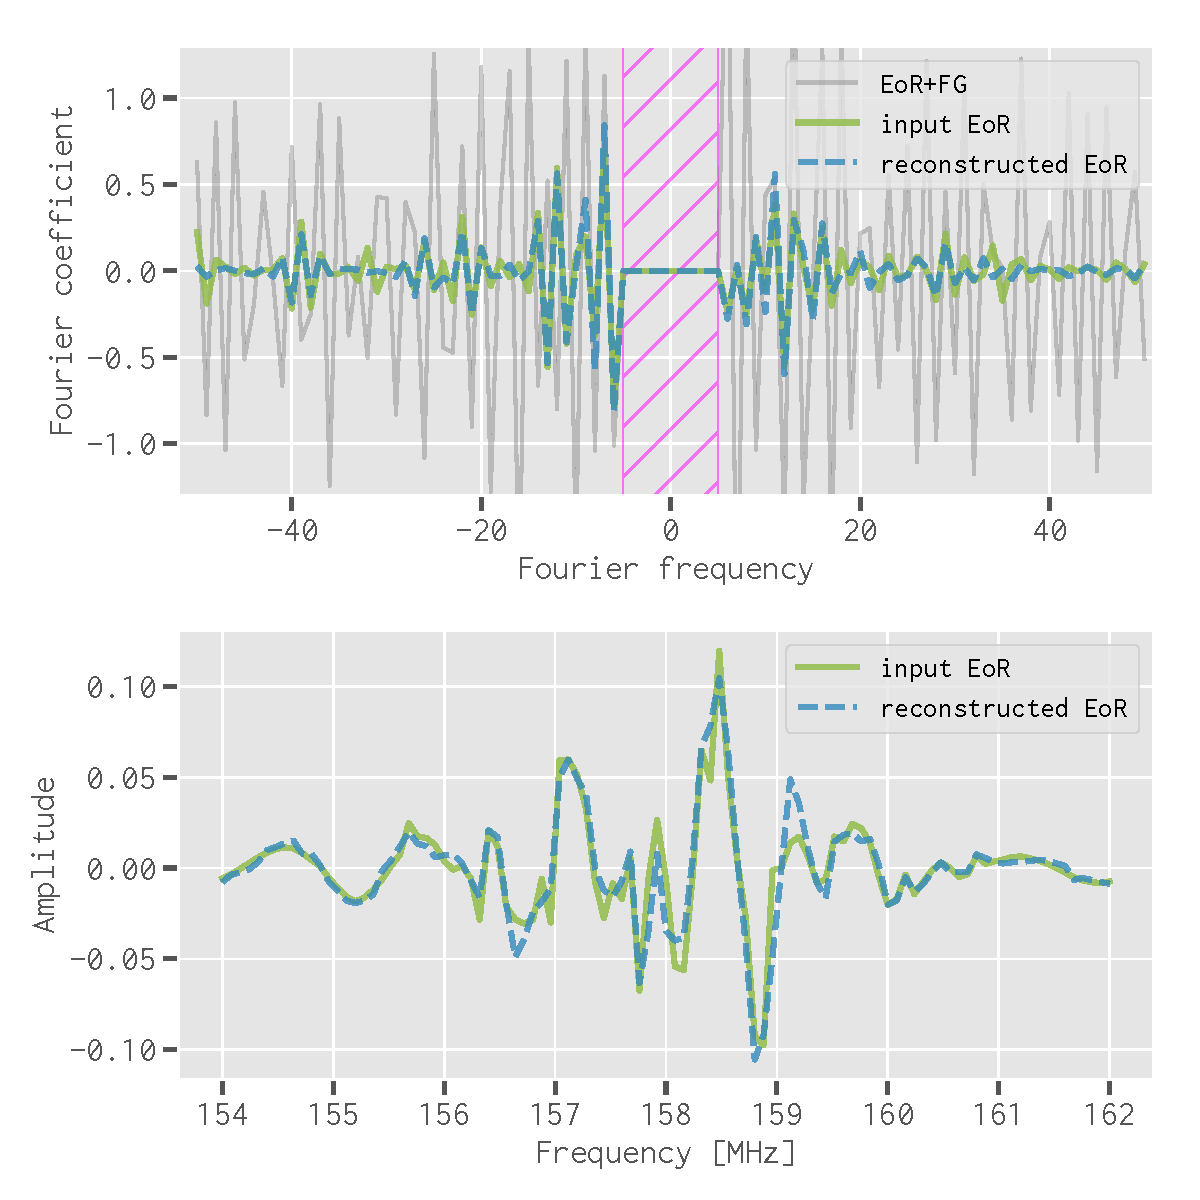
\includegraphics[width=0.9\textwidth]{cdae-eor-pix}
  \bicaption[CDAE 重建的 EoR 信号的示例]{%
    以\acl*{s-test} \ac*{s-test} 中一个随机像素点为例,
    展示了 CDAE 重建的和输入的 EoR 信号之间的对比.
    \uline{(上栏)}
    输入的 EoR 信号 $\B{x}_{\R{eor}}$ (绿色实线)
    和 CDAE 重建的 EoR 信号 $\B{r}_{\R{eor}}$ (蓝色虚线)
    在 Fourier 空间的对比.
    两个信号之间的\acl*{coef-correlation}为 $\ac*{coef-correlation} = 0.931$.
    图中的灰线表示输入的总辐射信号 $\B{x} = \B{x}_{\R{fg}} + \B{x}_{\R{eor}}$,
    品红阴影线标记的区域表示在 \autoref{sec:preprocessing}
    预处理过程中排除的 Fourier 系数.
    \uline{(下栏)}
    输入的 EoR 信号 $\B{x}_{\R{eor}}$ (绿色实线)
    和 CDAE 重建的 EoR 信号 $\B{r}_{\R{eor}}$ (蓝色虚线)
    变换回观测频率空间的对比.
  }{%
    An example of the EoR signal reconstructed by the trained CDAE for
    one random pixel in the test set \ac*{s-test}.
    \emph{(Upper)}
    The input EoR signal $\B{x}_{\R{eor}}$ (solid green line) and
    the reconstructed EoR signal $\B{r}_{\R{eor}}$ (dashed blue line)
    in the Fourier domain.
    The correlation coefficient between the input and
    reconstructed EoR signals is $\ac*{coef-correlation} = 0.931$.
    The gray line represents the input total emission
    $\B{x} = \B{x}_{\R{fg}} + \B{x}_{\R{eor}}$.
    The magenta hatched region marks the excised Fourier coefficients
    in data preprocessing (\autoref{sec:preprocessing}).
    \emph{(Lower)}
    The input EoR signal $\B{x}_{\R{eor}}$ (solid green line) and
    the reconstructed EoR signal $\B{r}_{\R{eor}}$ (dashed blue line)
    transformed back to the observing frequency domain.
  }
  \label{fig:cdae-eor-pix}
\end{figure}

\autoref{fig:cdae-train} 中还画出了\acl{loss-validation} \ac{loss-validation}
以及从\acl{s-validation} \ac{s-validation} 计算得到的评估指标
(即\acl{coef-correlation} \ac{coef-correlation})
随着 \ac{cdae} 训练过程的变化情况.
显然可见,损失 \ac{loss-training} 和 \ac{loss-validation} 均持续减小,
同时\acl{coef-correlation} \ac{coef-correlation} 稳步增长,
说明 \ac{cdae} 的训练效果很好而且没有出现\ac{overfitting}.
训练完成后,我们使用\acl{s-test} \ac{s-test} 来评估 \ac{cdae} 的性能,
可得 \ac{cdae} 重建的 EoR 信号与输入的 EoR 信号之间的
平均\acl{coef-correlation}达到了
$\bar{\xi}_{\R{cdae}} = \num{0.929 +- 0.045}$.
这个结果说明了训练好的 \ac{cdae} 在 EoR 信号的分离问题上取得了出色的成绩.
以\acl*{s-test} \ac*{s-test} 中一个随机像素点为例,
\autoref{fig:cdae-eor-pix} 展示了 CDAE 重建的和输入的 EoR 信号之间的对比
($\ac{coef-correlation} = 0.931$).

\begin{figure}[htp]
  \centering
  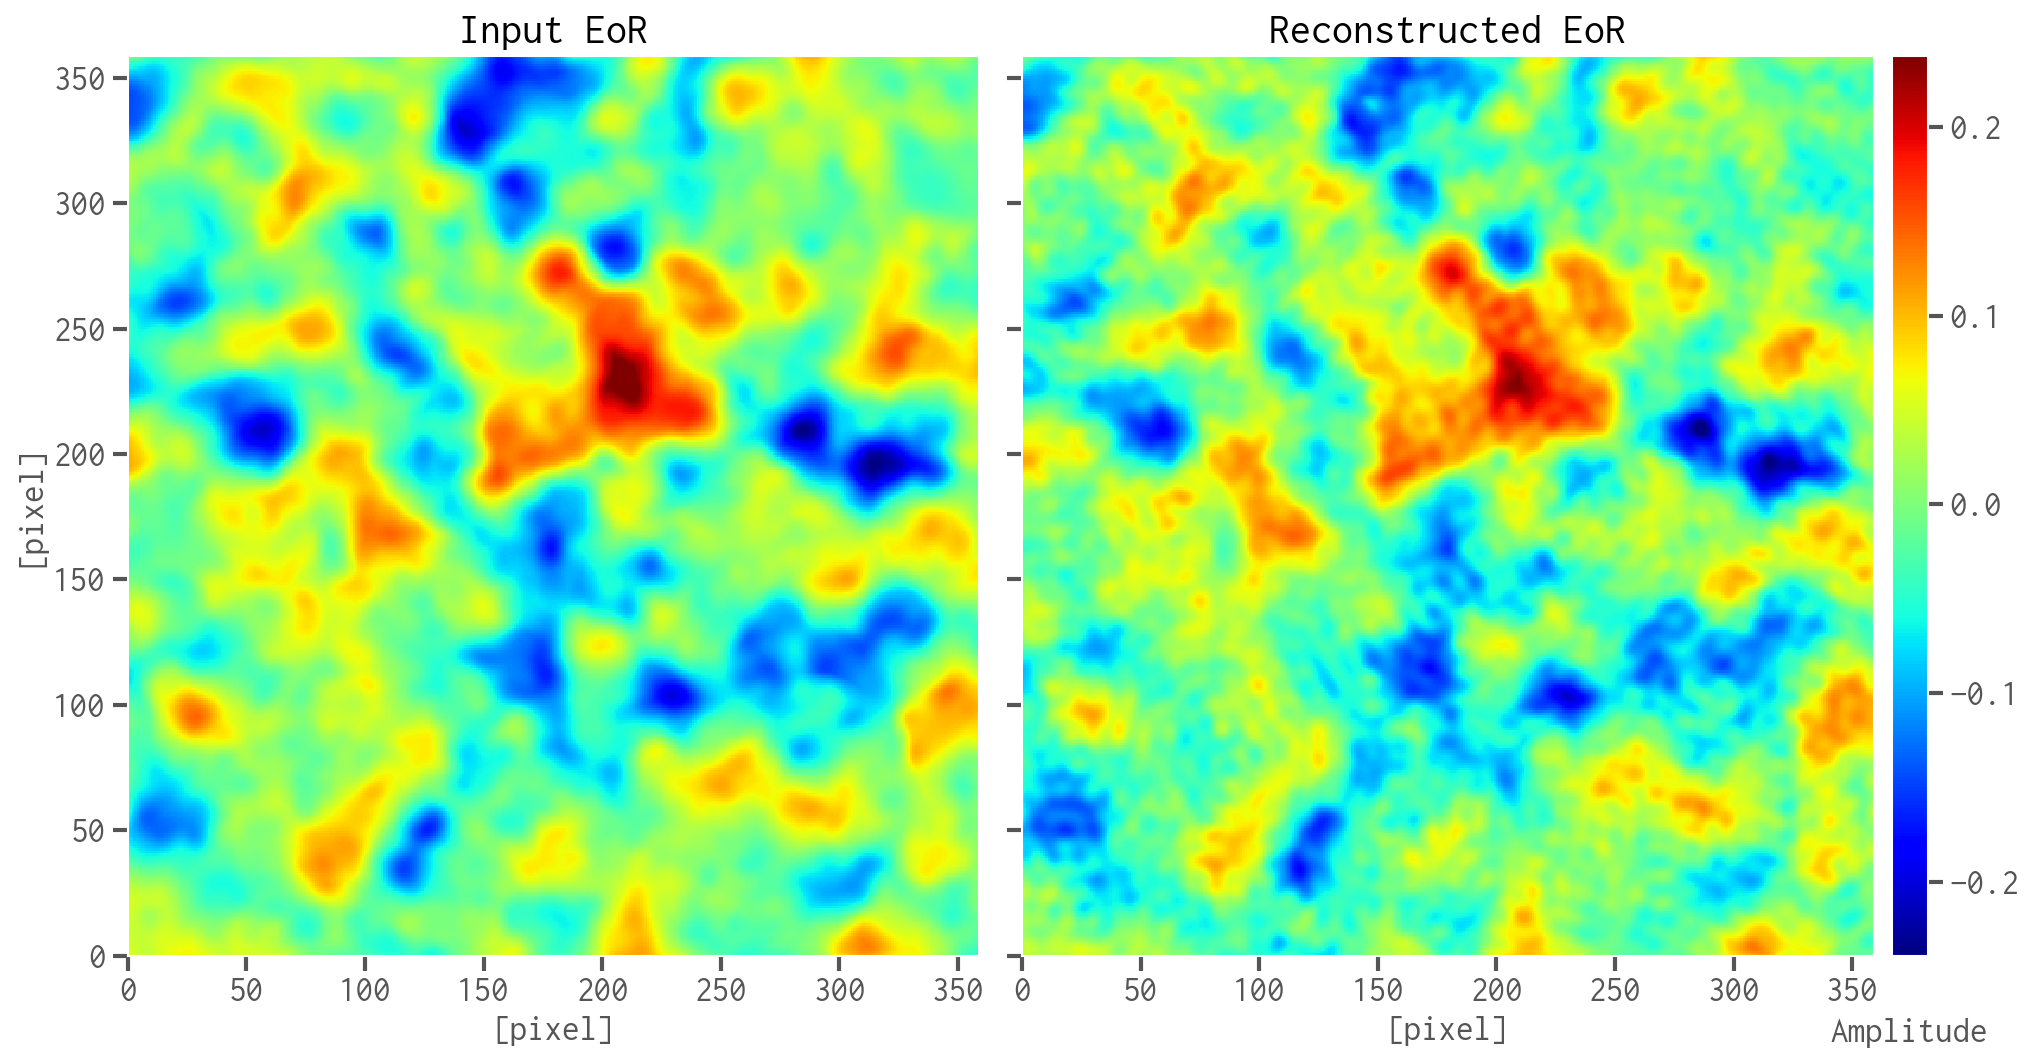
\includegraphics[width=\textwidth]{cdae-eor-img-comp}
  \bicaption[输入的 EoR 图像和 CDAE 重建的 EoR 图像的对比]{%
    输入的 EoR 图像(左栏)和 CDAE 重建的 EoR 图像(右栏)
    在中心频率 \SI{158}{\MHz} 处的对比.
    图像的尺寸均为 \num{360 x 360},并且使用了相同的\ac{colorbar},
    幅度因 CDAE 训练的需要已被标准化 (\autoref{sec:preprocessing}).
  }{%
    Comparison between the input EoR image (left panel) and
    reconstructed EoR image (right panel) at the central frequency of
    \SI{158}{\MHz}.
    The images have the same size (\num{360 x 360} pixel) and share the
    same color bar.
    The amplitude is normalized for the CDAE (\autoref{sec:preprocessing}).
  }
  \label{fig:cdae-eor-img}
\end{figure}

\begin{figure}[htp]
  \centering
  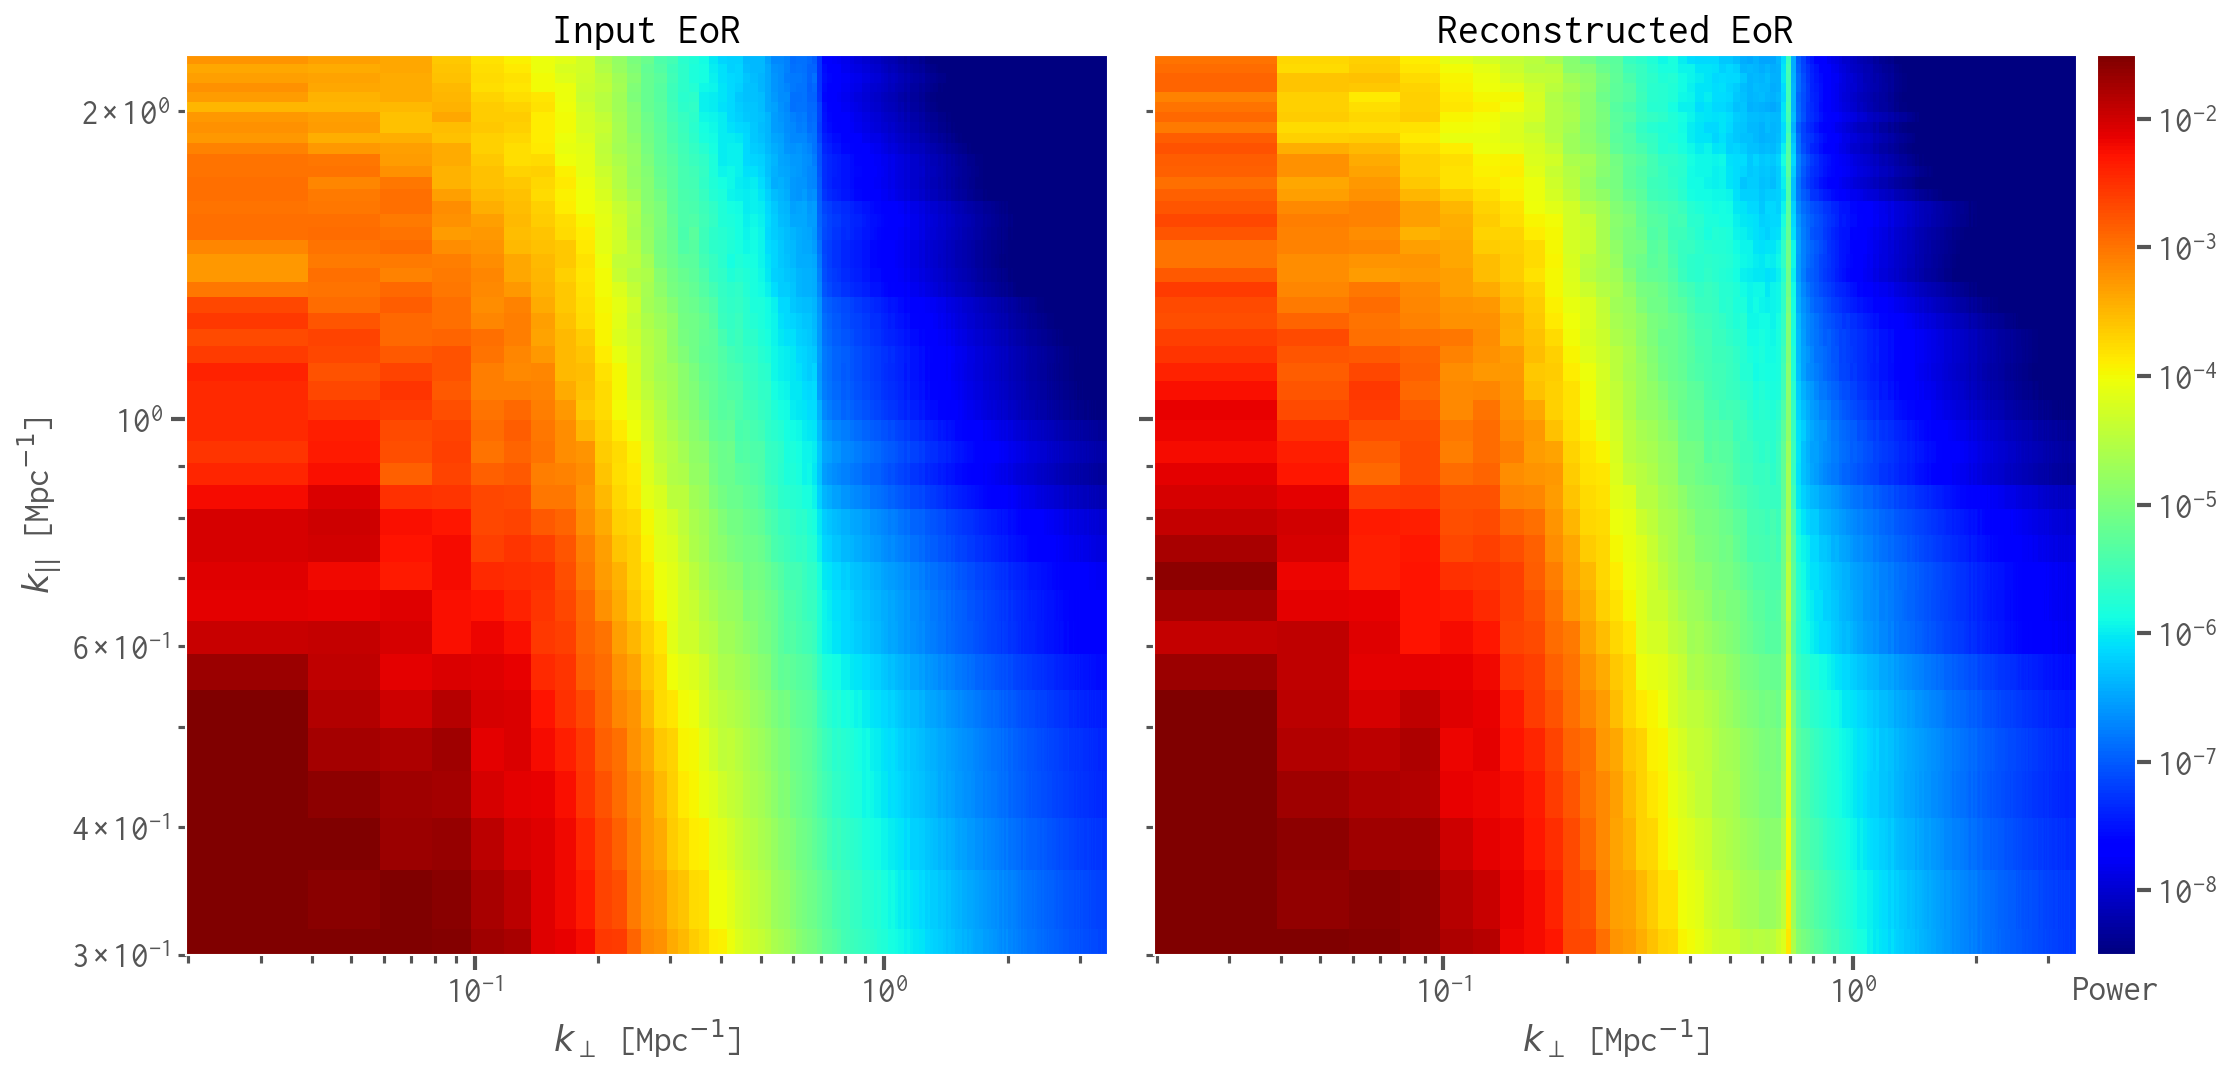
\includegraphics[width=\textwidth]{cdae-eor-ps-comp}
  \bicaption[输入的 EoR 信号和 CDAE 重建的 EoR 信号之间的二维功率谱对比]{%
    输入的 EoR 信号(左栏)和 CDAE 重建的 EoR 信号(右栏)之间的二维功率谱对比.
  }{%
    Comparison of two-dimensional power spectra between the input
    (left panel) and reconstructed (right panel) EoR signals.
  }
  \label{fig:cdae-eor-ps}
\end{figure}

由于\acl{s-test} \ac{s-test} 源自一对完整的\ac{imgcube}
$\left( C_{\R{eor}}^{(2)}, C_{\R{fg}}^{(2)} \right)$,
因此,在使用 \ac{s-test} 评估 \ac{cdae} 时我们能够获得
重建 EoR 信号的完整\ac{imgcube}用来进行图像和功率谱的对比.
以中心频率 \SI{158}{\MHz} 为例,如\autoref{fig:cdae-eor-img} 所示,
相比输入的 EoR 图像,由 \ac{cdae} 重建的 EoR 图像中存在一些微弱的小尺度波纹结构,
这些波纹的尺度约为 10 个像素点 ($\sim$\,\SI{200}{\arcsecond}),
源自数据预处理 (\autoref{sec:preprocessing}) 时去除了 $n_{\R{ex}} = 6$
个 Fourier 频率最小的系数.
除此之外,两张图像具有几乎完全相同的空间结构和强度分布.

另一方面,我们分别计算了输入的 EoR 信号和 \ac{cdae} 重建的 EoR 信号的二维\ac{ps},
结果如\autoref{fig:cdae-eor-ps} 所示.
在重建 EoR 信号的二维\ac{ps} 上,上面提及的小尺度波纹结构在
$\kperp \approx \SI{0.7}{\per\Mpc}$ 的尺度上贡献了额外的功率,形成了一条窄带.
在数据所覆盖的其他尺度上,\ac{cdae} 很好地恢复了 EoR 信号的功率.
此外,我们注意到两个二维\ac{ps}在 $\kperp \approx \SI{0.1}{\per\Mpc}$
的地方均有一条隐约可见的线,源自于有限长度的信号在进行 Fourier 变换时所产生的边界效应.

以上这些结果充分说明了训练好的 \ac{cdae} 能够有效地克服复杂的波束效应,
从强烈的前景干扰中准确地重建 EoR 信号.
\ac{cdae} 的优秀性能主要归功于堆叠多个卷积层所实现的强大的\ac{fx}能力,
这种堆叠式架构让每一层专注于提取相对简单的特征,
然后这些特征逐层地结合形成精细、抽象的高层次特征 \cite{leCun2015}.
同时,\num{53569} 个可训练的参数让 \ac{cdae} 拥有高度的灵活性.
经过有效训练后,\ac{cdae} 智能地从数据中学得一个针对 EoR 信号分离而优化的模型
\cite{domingos2012}.

%---------------------------------------------------------------------
\subsection{进一步验证}
\label{sec:cdae-validation}

\begin{figure}[htp]
  \centering
  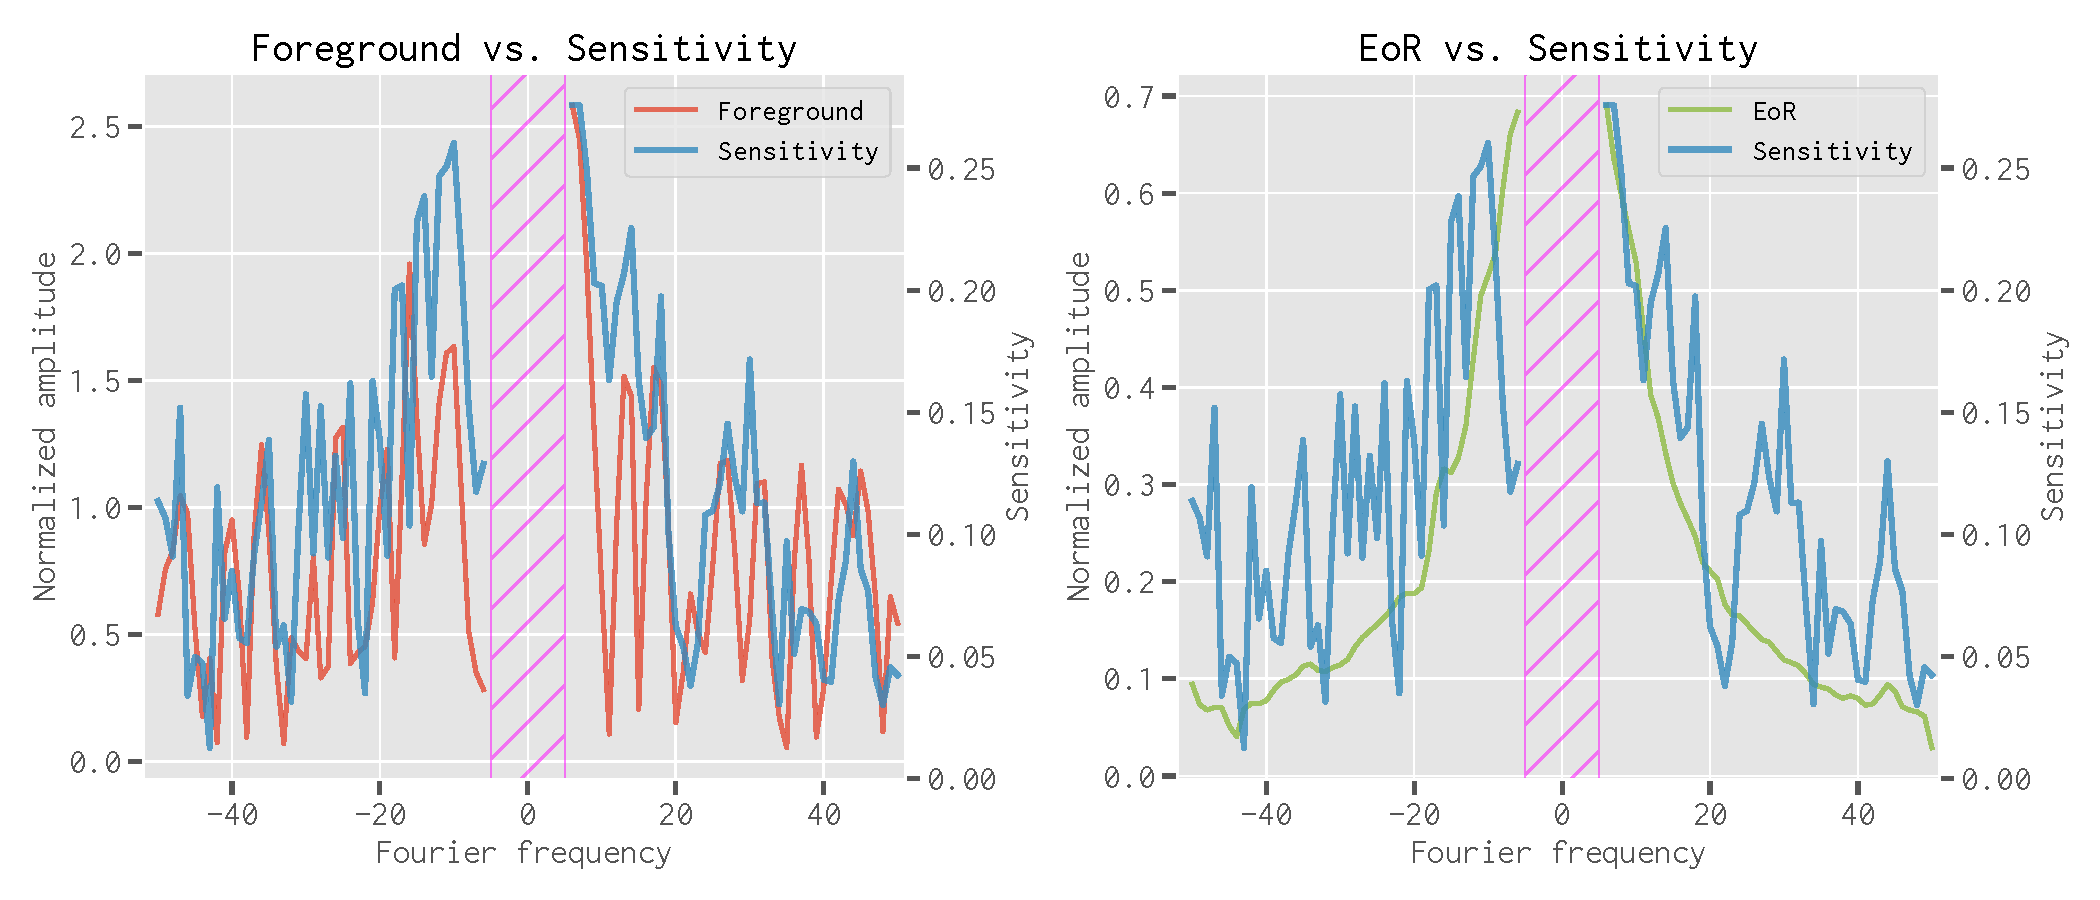
\includegraphics[width=\textwidth]{occlusion-fgeor}
  \bicaption[CDAE 对输入数据的灵敏度分布]{%
    采用\acs*{occlusion}方法得到的 CDAE 对输入数据的灵敏度分布 $\B{s}$ (蓝线).
    左图红线显示了前景辐射的强度的\acs*{rms}值 $\B{y}_{\R{fg}}$;
    右图绿线显示了 EoR 信号的强度的\acs*{rms}值 $\B{y}_{\R{eor}}$.
    通过计算\acl*{coef-correlation} \ac*{coef-correlation}
    可知灵敏度分布 $\B{s}$ 与 EoR 信号的相关性
    [$\ac*{coef-correlation}(\B{s}, \B{y}_{\R{eor}}) = 0.742$]
    显著大于与前景辐射的相关性
    [$\ac*{coef-correlation}(\B{s}, \B{y}_{\R{fg}}) = 0.562$].
  }{%
    The CDAE's sensitivity distribution $\B{s}$ (blue lines in both panels)
    obtained by applying the occlusion method.
    We also plot the root-mean-square amplitudes of
    the foreground emission $\B{y}_{\R{fg}}$ (red line in left panel)
    and the EoR signal $\B{y}_{\R{eor}}$ (green line in right panel).
    The sensitivity distribution $\B{s}$ is more correlated with
    the EoR signal
    [$\ac*{coef-correlation}(\B{s}, \B{y}_{\R{eor}}) = 0.742$]
    than the foreground
    [$\ac*{coef-correlation}(\B{s}, \B{y}_{\R{fg}}) = 0.562$].
  }
  \label{fig:occ-fgeor}
\end{figure}

为了进一步验证 \ac{cdae} 真正地从数据中发掘了 EoR 信号的有用特征,
我们采用\ac{occlusion}方法\cite{zeiler2014}
来可视化 \ac{cdae} 对输入数据的灵敏度的分布情况.
对\acl{s-validation} \ac{s-validation} 中的每一个输入信号 $\B{x}^{(i)}$,
遮挡其中连续的 3 个元素,记所得被遮挡的信号为 $\tilde{\B{x}}^{(i)}$,
然后输入训练好的 \ac{cdae},得到重建的 EoR 信号 $\tilde{\B{r}}^{(i)}_{\R{eor}}$.
如果输入信号 $\B{x}^{(i)}$ 没有被遮挡,
则 \ac{cdae} 重建的 EoR 信号为 $\B{r}^{(i)}_{\R{eor}}$.
对比在有无遮挡的两种情况下所重建的 EoR 信号的准确度,
于是可定义 \ac{cdae} 对输入数据被遮挡部分的灵敏度 $s$ 为:
\begin{equation}
  \label{eq:perf-loss}
  s = \frac{1}{N_{\R{val}}} \sum_{i=1}^{N_{\R{val}}} \left[
      \ac{coef-correlation} \left(
        \B{r}^{(i)}_{\R{eor}}, \B{x}^{(i)}_{\R{eor}}
      \right) -
      \ac{coef-correlation} \left(
        \tilde{\B{r}}^{(i)}_{\R{eor}}, \B{x}^{(i)}_{\R{eor}}
      \right)
    \right] ,
\end{equation}
其中 $\B{x}^{(i)}_{\R{eor}}$ 为输入的 EoR 信号,
$N_{\R{val}}$ 是\acl{s-validation} \ac{s-validation} 包含的数据点数目.
灵敏度 $s$ 越大,说明被遮挡的部分数据对 \ac{cdae} 的性能影响越强,
也就说明 \ac{cdae} 从该部分数据学到的特征越重要.

通过每次遮挡输入数据的不同部分并计算相应的灵敏度 $s$,
可以得到 \ac{cdae} 对输入数据各个部分的灵敏度分布 $\B{s}$,
如\autoref{fig:occ-fgeor} 所示.
图中还画出了前景辐射的强度的\acs*{rms}值 $\B{y}_{\R{fg}}$
以及 EoR 信号的强度的\acs*{rms}值 $\B{y}_{\R{eor}}$.
我们发现 \ac{cdae} 的灵敏度分布 $\B{s}$ 与 EoR 信号 $\B{y}_{\R{eor}}$
之间的相关性为 $\ac*{coef-correlation}(\B{s}, \B{y}_{\R{eor}}) = 0.742$,
显著高于与前景辐射 $\B{y}_{\R{fg}}$ 的相关性
[$\ac*{coef-correlation}(\B{s}, \B{y}_{\R{fg}}) = 0.562$].
这个结果表明,训练好的 \ac{cdae} 确实从输入数据中学到了
能够帮助区分前景辐射的 EoR 信号的特征,
因此,\ac{cdae} 对输入数据中\ac{snr}高的部分也更敏感.


%=====================================================================
\section{讨论}

%---------------------------------------------------------------------
\subsection{为什么使用 Fourier 变换预处理数据?}
\label{sec:why-ft}

为了说明使用 Fourier 变换预处理数据 (\autoref{sec:preprocessing}) 的优势,
我们开展了一次对比实验.
与 \autoref{sec:cdae-demo} 的演示唯一的区别是:
没有在数据预处理阶段运用 Fourier 变换.
我们使用相同的 \ac{cdae} 架构、\ac{ds}以及训练方法,
得到的训练结果如\autoref{fig:cdae-train-noft} 所示.
我们发现,\acl{loss-training} \ac{loss-training} 减小的速度更慢,
大约经过 100 个\ac{epoch}才收敛.
同时,从\acl{s-validation} \ac{s-validation}
计算得到的\acl{loss-validation} \ac{loss-validation} 以及
\acl{coef-correlation} \ac{coef-correlation}
的曲线上均有许多小\ac{spike},
表明 \ac{cdae} 的训练过程有一点不稳定.
这种现象在 \autoref{sec:cdae-demo} 的演示以及\autoref{fig:cdae-train}
中是没有的.
此外,使用\acl{s-test} \ac{s-test} 来评估 \ac{cdae} 的性能可得,
\ac{cdae} 重建的与输入的 EoR 信号之间的平均\acl{coef-correlation}仅有
$\bar{\rho}_{\R{noft}} = \num{0.628 +- 0.167}$,
显著差于 \autoref{sec:cdae-results} 的结果.

\begin{figure}[htp]
  \centering
  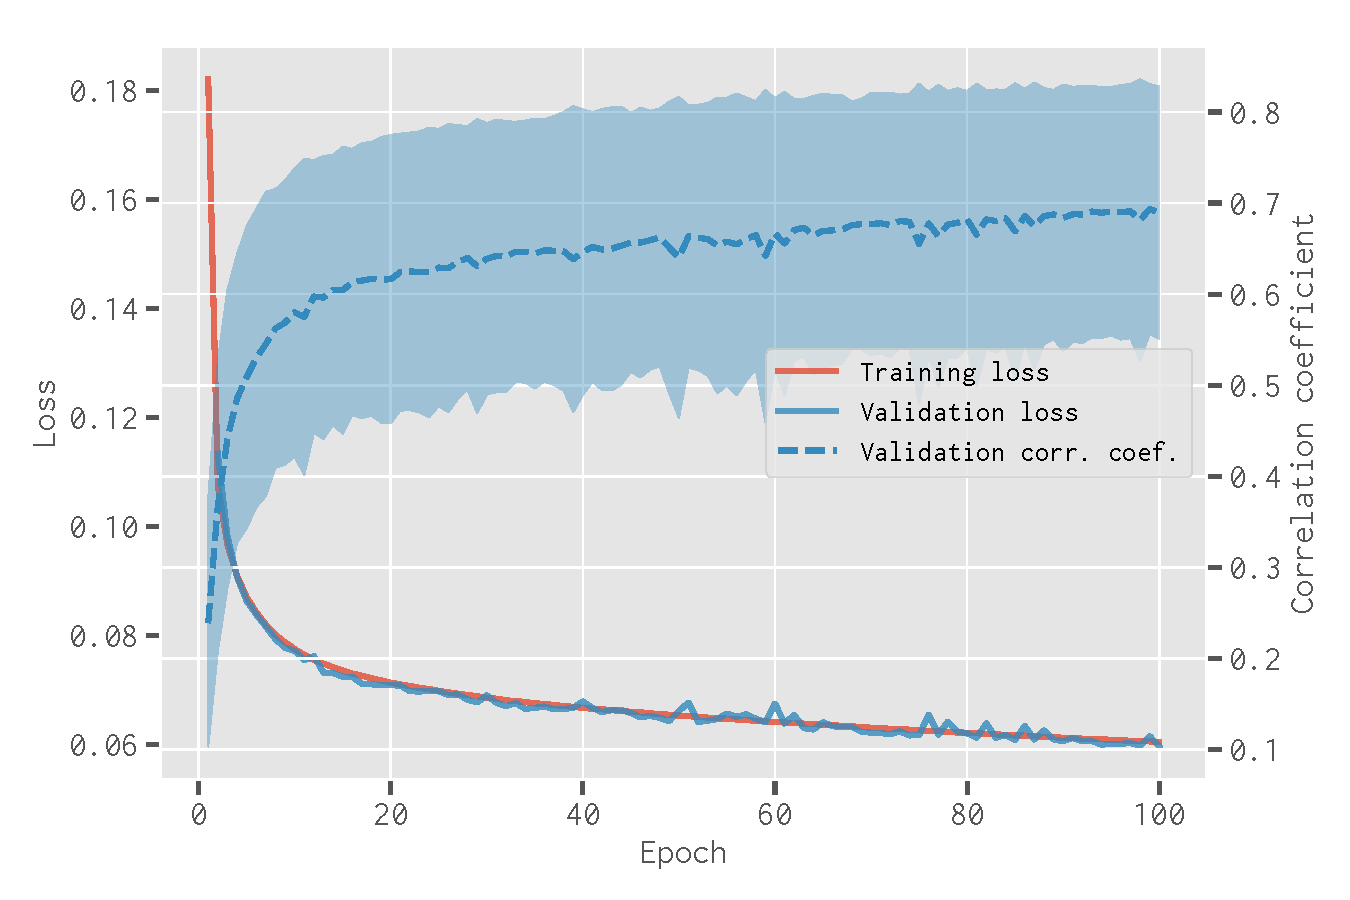
\includegraphics[width=\textwidth]{cdae-train-noft}
  \bicaption[在未使用 Fourier 变换预处理的数据集上训练 CDAE 得到的结果]{%
    CDAE 的训练过程和结果.
    与\autoref{fig:cdae-train} 类似,
    但是所用\acs*{ds}在预处理过程中没有运用 Fourier 变换.
  }{%
    The training process and result of the CDAE.
    Similar to Fig.~\ref{fig:cdae-train} but for the case that
    the data are preprocessed without applying the Fourier Transform.
  }
  \label{fig:cdae-train-noft}
\end{figure}

这些结果说明在\ac{ds}的预处理阶段运用 Fourier 变换是非常有帮助的.
将 EoR 信号和前景辐射的频谱信号变换到 Fourier 空间后,
EoR 信号主要分布在较大的 Fourier \ac{mode}里,
而频谱光滑的前景辐射则比较集中在较小的 Fourier \ac{mode}里 \cite{parsons2012},
所以两者的可区分度提高了,从而能够更准确地被 \ac{cdae} 学习并分离.

%---------------------------------------------------------------------
\subsection{与传统方法的对比}

如 \autoref{sec:fg-methods} 所述,
目前已有一批方法被提出来用于扣除强烈的前景污染从而分离出微弱的 EoR 信号,
这些\ac{fg-rm}方法可大致分为两类:参数化方法和非参数化方法.
为了进一步展示我们基于\ac{dl}设计的新算法的性能,
我们从传统的\ac{fg-rm}方法中挑选了两种典型的方法进行对比,
分别是多项式拟合法\cite{wang2006} 和\ac{cwt}法 \cite{gu2013}.
多项式拟合法因为简单、可靠而被广泛使用 \cite{jelic2008,liu2009ps,pritchard2010},
并且常常作为基准与其他\ac{fg-rm}方法对比 \cite{harker2009,alonso2015,chapman2015},
是参数化方法类别中最具代表性的一种方法.
在非参数化方法类别中,我们选取\ac{cwt}法是因为
该方法与 Wp 平滑法 \cite{harker2009}、\ac{gmca}法 \cite{chapman2013}
等其他非参数化方法性能相当,但是速度更快、使用更简单 \cite{gu2013,chapman2015}.

对于天空的每一个像素点 $i$,
多项式拟合法使用一个低阶多项式来拟合该像素点的总辐射的频谱
$\B{x}^{(i)} = \B{x}^{(i)}_{\R{eor}} + \B{x}^{(i)}_{\R{fg}}$,
确定其中的光滑成分,并作为前景扣除,从而分离出其中的 EoR 信号 \cite{wang2006}.
使用在 \autoref{sec:cdae-images} 模拟的\ac{imgcube}
$\left( C_{\R{eor}}^{(2)}, C_{\R{fg}}^{(2)} \right)$,
我们测试了从二阶到五阶的多项式,发现四阶多项式达到的 EoR 信号分离的效果最佳.
然而,使用四阶多项式拟合分离的 EoR 信号与输入 EoR 信号
之间的平均\acl{coef-correlation}仍然仅有
$\bar{\ac{coef-correlation}}_{\R{poly}} = \num{0.296 +- 0.121}$.
因此,当前景频谱的光滑性受到仪器的波束效应损坏时,多项式拟合法难以有效地扣除前景污染.

与其他\ac{fg-rm}方法一样,\ac{cwt}法同样依赖于前景辐射与 EoR 信号具有显著不同的频谱结构.
对于天空每一个像素点的总辐射的频谱,首先运用基于 Morlet 小波函数的\ac{cwt},
于是前景辐射和 EoR 信号因为频谱特征不同而在小波空间中占据不同的区域.
在小波空间中,可以更容易地识别那些主要源自前景辐射的小波系数并将其扣除,
然后再逆变换回观测频率空间,便得到已扣除前景污染的 EoR 信号 \cite{gu2013}.
使用相同的\ac{imgcube}
$\left( C_{\R{eor}}^{(2)}, C_{\R{fg}}^{(2)} \right)$,
我们通过调节\ac{cwt}法的参数以达到最佳的性能.
于是,我们最终采用的参数为:
最小缩放因子 $s_{\R{min}} = 7.4$,
最大缩放因子 $s_{\R{max}} = 50.0$,
缩放级数 $n_{\R{scale}} = 50$,
以及\ac{coi} $c_i = 1.6$.
但是,\ac{cwt}法分离的 EoR 信号与输入 EoR 信号之间的平均\acl{coef-correlation}仅有
$\bar{\ac{coef-correlation}}_{\R{cwt}} = \num{0.198 +- 0.160}$.
这个分离结果相比上述多项式拟合法的结果还要稍差一点,
这与 \citeay{gu2013} 的对比结果不同.
主要原因是我们模拟的\ac{imgcube}的频带更窄、频率分辨率更差,
所以在使用\ac{cwt}时产生了更严重的边界效应.

总之,干涉阵列的复杂波束效应使前景辐射的频谱产生了小尺度涨落,
破坏了前景辐射的频谱光滑性 [参见\autoref{fig:cdae-simdata}(b)].
于是,低阶多项式无法有效拟合前景辐射的频谱,
在小波空间中区分前景辐射和 EoR 信号也变得非常困难,
因此上述两种传统的\ac{fg-rm}方法都难以对复杂的前景辐射建模并扣除,
导致分离的 EoR 信号的准确度都比较低.
\ac{cdae} 则完全不同.
凭借强大的\ac{fx}能力以及数据驱动 (data-driven) 的特点,
\ac{cdae} 可以从训练数据中汲取信息来优化自身模型,
实现 EoR 信号与波束效应所导致的前景频谱的涨落之间的区分.
因此,\ac{cdae} 能够准确地分离 EoR 信号,取得非常出色的性能.


%=====================================================================
\section{小结}

The frequency-dependent beam effects of interferometers can cause
rapid fluctuations along the frequency dimension,
which damage the smoothness of the foreground spectra and prevent
traditional foreground removal methods from uncovering the EoR signal.
Given the difficulties in crafting practicable models to overcome the
complicated beam effects, methods that can intelligently learn tailored
models from the data seem more feasible and appealing.
To this end, we have proposed a deep-learning-based method that uses
a 9-layer CDAE to separate the EoR signal.
The CDAE has been trained on the simulated SKA images and has achieved
excellent performance.
We conclude that the CDAE has outstanding ability to overcome the
complicated beam effects and accurately separate the faint EoR signal,
exhibiting the great potential of deep-learning-based methods
to play an important role in the forthcoming EoR experiments.

本章内容已发表于 \mnras{} (MNRAS) \cite{li.cdae}.


%% EOF
